%
% TODO:
%% - add figures of histograms of EC attack

\chapter{Quantum digital signatures}\label{chapter:qds}
%Goal of chapter: introduce our QDS protocol and prove its security in different contexts using several methods.


In this chapter we introduce and investigate a continuous-variable Quantum Digital Signatures (QDS) protocol, which allows for secure authentication of classical messages even against a quantum adversary. We describe the protocol and its similarities and differences to recent QDS protocols from the literature in Sec.~\ref{sec:qds_protocol}, and then prove its security against several different attack strategies in Secs.~\ref{sec:qds_security_repudiation}-\ref{sec:qds_attack_analysis}. It is only recently that QDS protocols in the discrete-variable regime have been proven secure against and eavesdropping attack on the quantum channels \cite{Amiri2016, Yin2016}, and the work in this chapter marks the first time that continuous-variable QDS is proven secure against an eavesdropper. Finally, in Secs.~\ref{sec:qds_siglength}-\ref{sec:qds_protocol_performance} we analyse the performance of our protocol, including a postselection technique to improve performance, and demonstrate that a remarkably small number of quantum states are required to securely sign a message. Our protocol is implemented in Chapter~\ref{chapter:aqc}.

\section{Our QDS protocol}\label{sec:qds_protocol}

In the simplest instance we may consider a signature scheme involving only three parties: a sender, Alice ($A$), and recipients Bob ($B$) and Charlie ($C$). Alice wishes to send a classical message $m$ to $B$ and $C$, such that $B$ and $C$ can correctly determine whether $m$ was indeed sent by $A$. Furthermore the recipients should be able to check whether $m$ has been altered. The three-party setting is the smallest setting to fully distinguish a digital signatures protocol from related protocols such as MACs\footnote{Message Authentication Codes. See Ref.~\cite{Schneier1996}.}. Because more than two (potentially dishonest) players are present, this allows for new attack strategies which distinguish QDS from other quantum tasks such as QKD.

\subsection{QDS setup}

\begin{figure}[htp]
\centering

\includegraphics[width=\linewidth, draft=false]{qds/qds_cartoon}
\caption{\label{fig:qds_cartoon} Setup of a $3$-party digital signatures scheme. Alice (A) wishes to securely sign her message $m$ such that Bob (B) and Charlie (C) both accept it as genuine.}
\end{figure}

Our signature scheme is displayed pictorially in Fig.~\ref{fig:qds_cartoon}. Alice (A) wishes to send a message $m$ to Bob (B) and Charlie (C) such that both Bob and Charlie accept it as genuine. To accomplish this she appends to $m$ a signature $\sigma_m$ which should be unique to the message and uniquely generated by Alice. In this way our digital signatures scheme is a quantum generalization of Lamport's protocol \cite{Lamport1979, Schneier1996}. As we shall see later, any player in our protocol may be dishonest.

\subsection{Goals of a signature scheme}\label{sec:qds_goals}




\begin{mylist}[htp]
\captionsetup{width=0.8\linewidth}
\begin{framed}
\begin{enumerate}
\item\emph{Security against forgery}, Fig.~\ref{fig:attacks_forgery}. Neither a dishonest recipient ($B$ or $C$), nor an external fourth party (Eve, $E$), should be able to alter $m$ and have it accepted as genuine by an honest recipient. The signature scheme should ensure that $m$ is the message which Alice sent.

\item\emph{Genuine sender}, Fig.~\ref{fig:attacks_forgery}. Neither a dishonest recipient ($B$ or $C$), nor an external fourth party (Eve, $E$), should be able to impersonate $A$. Any message which falsely claims to have originated with Alice should be rejected.

\item\emph{Security against repudiation}, Fig.~\ref{fig:attacks_repudiation}. A dishonest sender $A$ should not be able to cause disagreement between $B$, $C$ about the previous two requirements. After genuinely sending $m$ she should not later be able to deny it, and if Bob accepts the message as genuine then so too should Charlie. 

\item \emph{Message transferability}, Fig.~\ref{fig:attacks_repudiation}. If $B$ accepts a message as genuine, then he should be sure that $C$ will also accept.

\item \emph{Robustness}, Fig.~\ref{fig:attacks_robustness}. The message $m$ should be accepted if all players behave honestly and there is no tampering by an eavesdropper.
\end{enumerate}
\caption{\label{list:qds_requirements} A secure QDS scheme should fulfill each of the above requirements. Requirement $1$ implies requirement $2$. In our $3$-party setting, requirements $3$ and $4$ are equivalent. We depict each type of attack which a QDS scheme must prevent in Fig.~\ref{fig:qds_attacks}.}
\end{framed}
\end{mylist}


%Requirements $1$ and $2$ are fulfilled in our scheme by the same security process, and so we will focus on $1$ and simply note where $2$ arises.

A digital signature scheme must fulfill the requirements outlined in List.~\ref{list:qds_requirements}. If requirement $1$ (security against forgery) holds then no dishonest player will be able to impersonate Alice, which fulfills requirement $2$ (genuine sender). In order to do so they will be required to generate $\sigma_m$ which at the start of the protocol is known only to her. The dishonest player's only hope for successful impersonation is to take Alice's place at the start of the protocol and perform a so-called ``man-in-the-middle'' attack. We do not investigate this possibility further, though we note that without previous authenticated interaction between players even QKD is insecure for this attack \cite{Broadbent2015}.

For our scheme involving three parties, requirements $3$ and $4$ are equivalent. A QDS protocol involving $N$ recipients may distinguish between non-repudiation and transferability by defining a message $m^{\left(k\right)}$ as $k$-transferable if it may be successfully forwarded up to $k$ times. An honest participant should be able to determine the transferability level of $m$ \cite{Arrazola2015}, while non-repudiation then refers to Alice's ability to cause a message to be non-transferable. In what follows we treat these requirements as equivalent.

A digital signature scheme which rejects all messages trivially fulfills requirements $1-4$, and so in order to get a useful digital signature scheme we must also impose requirement $5$.

\begin{figure}[htp]
\captionsetup{width=0.8\linewidth}
\centering
	\begin{subfigure}{\linewidth}
		\centering
		
\includegraphics[draft=false, width=\linewidth]{qds/qds_cartoon_forgery}
		\caption{\label{fig:attacks_forgery}}
	\end{subfigure}
	\begin{subfigure}{\linewidth}
		\centering
		
\includegraphics[draft=false, width=\linewidth]{qds/qds_cartoon_repudiation}
		\caption{\label{fig:attacks_repudiation}}
	\end{subfigure}
	\begin{subfigure}{\linewidth}
		\centering
		
\includegraphics[draft=false, width=\linewidth]{qds/qds_cartoon_honest_failure}
		\caption{\label{fig:attacks_robustness}}
	\end{subfigure}
\caption{\label{fig:qds_attacks} The multipartite setting permits many different methods for attack on the protocol depicted in Fig.~\ref{fig:qds_cartoon}. Gray boxes depict honest players while red boxes depict dishonest players. (a) Forging attack with dishonest Bob. Bob will change the message $m \rightarrow n$ with fake signature $\sigma_n$. The attack succeeds if Charlie accepts. Alternatively, either Charlie or a fourth player, Eve, may attempt a forging attack against an honest player. (b) Repudiation attack with dishonest Alice. Alice tries to convince Bob to accept the message and Charlie to reject it. (c) Honest failure: all players behave honestly but the protocol fails and both Bob and Charlie reject $m$. A protocol which does not fail due to honest failure is called robust.}
\end{figure}

\FloatBarrier
\subsection{QDS protocol description}

We here present a continuous-variable (CV) QDS protocol based on the quadrature phase-shift keying (QPSK) alphabet of coherent states, Fig.~\ref{fig:qpsk}. For the first time in a continuous-variables QDS protocol, our protocol takes into account insecure quantum distribution channels and permits the presence of an eavesdropper. Surprisingly, the same step of the protocol which ensures security against eavesdropping also makes the protocol efficient in its use of quantum resources. We shall see later in Sec.~\ref{sec:qds_protocol_performance} that we outperform recent comparable QDS protocols.

\begin{figure}[htp]
\captionsetup{width=0.8\linewidth}
\centering
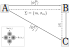
\includegraphics[draft=false, width=\linewidth]{qds/qds_setup}
\caption{\label{fig:qds_setup} Setup of the QDS protocol considered in this chapter. Alice (A) wishes to securely sign a $1$~bit message $m$. Alice distributes quantum coherent states $\ket{\phi_j^{\left(B, C\right)}}$ along insecure quantum distribution channels (solid lines) during the Distribution stage. Bob and Charlie swap eliminated signature elements via their securely encrypted classical channel (dotted lines). During the Messaging stage Alice sends $\Sigma$, containing her message $m$ and her corresponding signature $\sigma_m$ along a classical broadcast channel (dot-dashed line). Inset: QPSK alphabet.}
\end{figure}


Our QDS scheme is split into two stages, Distribution and Messaging, which, by analogy with classical digital signatures, may occur with significant time delay. Quantum states are sent and measured during Distribution. During Messaging Alice will send her message and classical signature, and recipients Bob and Charlie will try to determine its validity.\footnote{Note the intrinsic separation between the Distribution (quantum) and Messaging (classical) stages of the protocol. We will take further advantage of this separation between quantum and classical steps in Chapter~\ref{chapter:aqc}} Our protocol setup is outlined in Figs.~\ref{fig:qds_cartoon},~\ref{fig:qds_setup}. 
\par
\noindent We will now describe in detail the running of the protocol.



\subsubsection{Distribution stage}

\paragraph{Step $1$.}
Alice wishes to send a signed $1$ bit message $m$ to Bob and Charlie. For each possible future $m$, and for each recipient, Alice creates the following classical strings
\begin{equation}
\Phi_m^{\left(B, C\right)} = \left\{ \phi_{j, m}^{\left(B, C\right)}\right\}_{j=1}^{L}
\end{equation}
which are of length $j$. The $\phi_{j}$ are complex phases chosen uniformly at random from the QPSK alphabet. The strings $\Phi_m^{\left(B, C\right)}$ may be interpreted as Alice's \emph{private key}. The signature length $L \in \mathbb{N}$ is chosen to ensure the desired level of security.

\paragraph{Step $2$.} Corresponding to each private key, Alice forms the following quantum states
\begin{equation}\label{eqn:QDS_publickey}
\rho\left[\Phi_m^{\left(B, C\right)}\right] := \otimes_{j=1}^L \; \rho\left[\phi_{j, m}^{\left(B, C\right)}\right]
\end{equation}
with
\begin{equation}
\rho\left[\phi_{j, m}^{\left(B, C\right)}\right] := \ket{\phi_{j, m}^{\left(B, C\right)}} \bra{\phi_{j, m}^{\left(B, C\right)}} \notag
\end{equation}
understood to be the coherent state from QPSK with phase corresponding to the relevant element of Alice's private key.

The states Eq.~\ref{eqn:QDS_publickey} may be interpreted simply as sequences of coherent states, and correspond to Alice's \emph{public key}. An important difference between quantum and classical digital signatures is that here the public key may no longer be freely distributed, copied and stored. We also note that Alice no longer has a single public key for each message (unlike Lamport's scheme \cite{Lamport1979}), and her quantum public key differs both for each possible $m$ and for each recipient (unlike the recent scheme Ref.~\cite{Croal2016}). This is a requirement for security against an eavesdropping forger, Sec.~\ref{sec:qds_security_forgery}.

\paragraph{Step $3$.}
Each recipient $B, C$ performs heterodyne detection on their received coherent states, and receives outcomes $\left( \qout, \pout \right)$ which we will write as $z = \qout + i \pout \in \mathbb{C}$. Crucially, since measurement is performed immediately on receipt of the states no quantum memory is required. The remainder of the protocol is entirely classical.


At the end of the quantum stage of the protocol, recipients Bob and Charlie now possess classical strings, length $L$, containing their phase measurements on Alice's distributed states. They now form \emph{eliminated signatures}, Fig.~\ref{fig:elimsig}. For each $z \in\mathbb{C}$, recipients record the phases $\phi_{j, m}^{\left(B, C\right)}$ which Alice was \emph{least likely} to have sent. At position $j$ this may be understood as computing the four conditional probabilities 
\begin{equation}
p\left(\phi_j \given x_j\right) \qq{for each phase} \phi_j \in \text{QPSK},
\end{equation}
and recording the two $\phi_j$ which yield the smallest of these. This record of $\phi_j$ forms the $j^{\text{th}}$ element of their eliminated signatures. We note that the $\phi_j$ comprising the eliminated signature element will always be adjacent in phase space, and an example of this elimination procedure is displayed in Fig.~\ref{fig:elimsig}. We denote Bob and Charlie's total eliminated signatures at this stage as $X_m^{\left(B, C\right)}$. Each is of length $L$ and they will later be compared to Alice's private key in order to test the validity of the message. We display the possible eliminated signature elements and their requisite heterodyne outcomes in Tab.~\ref{tab:elimsig}.

\begin{figure}[htp]
\captionsetup{width=0.8\linewidth}
\centering
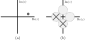
\includegraphics[draft=false, width=\linewidth]{qds/elimsig}
\caption{\label{fig:elimsig} Bob and Charlie each perform heterodyne measurement on their received coherent states, and obtain $\left(\qout, \pout\right)$. We define $z = \qout + i \pout$, which is the dark gray circle in (a). From their $z$, Bob and Charlie then record the two states from QPSK which are least likely to have been sent by Alice, (b). We display the possible eliminated signature elements and their requisite heterodyne outcomes in Tab.~\ref{tab:elimsig}.}
\end{figure}


\begin{table*}
\captionsetup{width=0.8\linewidth}
\centering \ra{1.75}
\begin{tabular*}{\linewidth}{@{\extracolsep{\stretch{1}}} c c c}

\head{Element} & \head{QPSK elements} & \head{Heterodyne outcome} \\ 
\hline 
$e_1$ & $\ket{- \phantom{i}\alpha}, \ket{- i \alpha}$ & $\qout >0, \pout >0$ \\ 

$e_2$ & $\ket{- i \alpha}, \ket{\phantom{-i}\alpha}$ & $\qout < 0, \pout > 0$ \\ 

$e_3$ & $\ket{\phantom{-i}\alpha}, \ket{\phantom{-}i \alpha}$ & $\qout < 0, \pout < 0 $ \\ 

$e_4$ & $\ket{\phantom{-}i \alpha}, \ket{- \phantom{i} \alpha}$ & $\qout > 0, \pout < 0$ \\ 
%\hline
\end{tabular*} 
\caption{\label{tab:elimsig} We denote possible eliminated signature elements as $e_1, e_2, e_3, e_4$, and display their corresponding states from QPSK and their requisite heterodyne measurement outcomes.}
\end{table*}



\paragraph{Step $4$. \emph{Symmetrization:}}
Bob and Charlie now swap a random $L/2$ elements of their $X_m^{\left(B, C\right)}$ over their encrypted classical channel. Signature elements which have been forwarded by a player will no longer be used by him in the protocol. We denote these resulting strings as $Y_m^{\left(B, C\right)}$. By using an encrypted classical channel the positions and values of swapped elements are kept secret from Alice, which will ensure that the information which Bob and Charlie each hold is symmetric from Alice's point of view \cite{Dunjko2014, Wallden2015}. 

In other words, at the end of Step~$3$, having sent the state $\ket{\phi_{j, m}^B}\bra{\phi_{j, m}^B}$ to Bob, Alice knows that Bob holds the corresponding eliminated signature element $X_{j, m}^B$, even though she doesn't know its value. Since Alice knows which state she sent to Bob, she may gain an advantage in trying to guess $X_{j, m}$. At the end of Step~$4$ however, Alice does not know whether it is Bob or Charlie who holds $X_{j, m}^B$. This uncertainty will prove crucial for preventing successful repudiation.

Bob (Charlie) now possesses an eliminated signature $\tilde{X}_m^{\left(B\right)}$ in two halves: one half $Y_m^{\left(B\right)}$ ($Y_m^{\left(C\right)}$) containing those elements received directly from Alice, and one half $Z_m^{\left(B\right)}$ ($Z_m^{\left(C\right)}$) containing elements received during this Symmetrization step from Charlie (Bob).

The key parameters for the Distribution stage are the signature length $L$, which directly measures the quantum resources required for the protocol, and the alphabet parameter $\alpha$, related to the average photon number of the distributed coherent states. Channel parameters such as loss and thermal noise will be discussed later\footnote{In Appendix~\ref{appendix:qds_larger_alphabets} we discuss an extension to the protocol which allows it to run with an $N$PSK alphabet of coherent states, where $N$ is an even integer.}.


\subsubsection{Messaging stage}

Messaging may occur at any time after Distribution.

\paragraph{Step $5$.}
To sign $m$, Alice sends to Bob the classical information $\Sigma = \left(m, \sigma_m\right)$, consisting of the message $m$ which she would like to convey, and her private key $\sigma_m = \left(\Phi_m^B, \Phi_m^C\right)$ consisting of declared phases, which acts as $m$'s signature. 


\paragraph{Step $6$.} Bob rearranges $\sigma_m \rightarrow \tilde{\sigma}_m^B := \left(\tilde{\Phi}_{Y, m}^B, \tilde{\Phi}_{Z, m}^B\right)$ by selecting elements from Alice's declaration which correspond to the two halves of his eliminated signature $\tilde{X}_m^{\left(B\right)}$. The original $\sigma_m$ has length $2 L$, while $\tilde{\sigma}_m^B$ has length $L$.

Bob compares relevant elements of $\tilde{\sigma}_m^B$ to his $\tilde{X}_m^{B}$, choosing which half of $\tilde{X}_m^B$ to compare to based on whether he kept or swapped the eliminated signature element. Bob makes a decision about whether to accept $m$ as genuine based on the number of \emph{mismatches} between Alice's signature and his own eliminated signatures. A mismatch is defined below in Sec.~\ref{sec:qds_mismatches} and in Fig.~\ref{fig:qds_mismatches}.


If Bob measures fewer than $s_B L/2$ mismatches on both of his eliminated signature halves then he accepts Alice's message as genuine, otherwise the protocol aborts. Bob's threshold mismatch rate $s_B$ determines how many mismatches he can observe before a signature fails his check. In general, $s_B$ is a free parameter of the protocol and will be discussed further in Secs.~\ref{sec:qds_mismatches},~\ref{sec:qds_security_repudiation},~\ref{sec:qds_siglength}.

%If Bob measures sufficiently few mismatches on both of his eliminated signature halves
%, i.e. if $\mathcal{M}\left(\tilde{\Phi}_{Y, m}^B, Y_m^B\right) < s_B L/2$ and $\mathcal{M}\left(\tilde{\Phi}_{Z,m}^B, Z_m^B\right) < s_B L/2$ 
%then he accepts Alice's declaration $m$ as genuine, otherwise the protocol aborts. %The threshold $0 \le s_B \le 1$ is related to the security of the protocol and will be discussed later.

\paragraph{Step $7$.} If Bob has accepted $m$, then he forwards $\Sigma$ to Charlie, who similarly checks for mismatches between Alice's signature and his eliminated signature. Charlie accepts the message if %$\mathcal{M}\left(\tilde{\Phi}_{Y, m}^C, Y_m^C\right) < s_C L/2$ and $\mathcal{M}\left(\tilde{\Phi}_{Z, m}^C, Z_m^C\right) < s_C L/2$, with security threshold $0 \le s_c \le 1$ to be discussed later. 
there are fewer than $s_C L/2$  mismatches between $\tilde{\sigma}_m^C$ and $\tilde{X}_m^{\left(C\right)}$. If Charlie also accepts $m$ then the protocol has succeeded, otherwise it aborts.  Charlie's threshold mismatch rate is $s_C$ and will be discussed further in Secs.~\ref{sec:qds_mismatches},~\ref{sec:qds_security_repudiation},~\ref{sec:qds_siglength}.

The key parameters for the Messaging stage are $s_B, s_C$ which may be freely chosen by Bob and Charlie in order to optimize security. We observe in Sec.~\ref{sec:qds_security_repudiation} that the choice $s_B \le s_C$ will ensure security against Alice's repudiation attack.

%\clearpage
\subsection{Counting mismatches}\label{sec:qds_mismatches}

\begin{figure}[htp]
\captionsetup{width=0.8\linewidth}
\centering
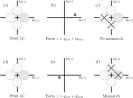
\includegraphics[draft=false, width=\linewidth]{qds/mismatch1}
\caption{\label{fig:qds_mismatches} A mismatch occurs when an honest party eliminates the state which Alice claims to have sent. (a, d) Alice sends coherent state $\ket{\alpha}$. (b, e) Bob (Charlie) heterodynes and receives $\left(\qout, \pout\right)$. We define $z = \qout + i \pout$. Even when all players are honest there is some probability of measuring $\qout < 0$, Sec.~\ref{sec:qds_modelling_perr}. (c) The eliminated signature element consists of $\ket{- \alpha}, \ket{- i \alpha}$ so there is no mismatch. (f) The eliminated signature element consists of $\ket{\alpha}, \ket{i \alpha}$ and so there is a mismatch.}
\end{figure}


The key test of validity which our protocol employs is a check on the number of mismatches between Bob or Charlie's eliminated signatures $\tilde{X}^{\left(B, C\right)}_m$ and Alice's declaration $\sigma_m$. A mismatch occurs if the state which Alice claims to have sent has been eliminated, Fig.~\ref{fig:qds_mismatches}. 

To be concrete, a mismatch occurs at position $j$ if
\begin{equation}
\phi_{j, m}^{B \left(C\right)} \in Y_{j, m}^{B \left(C\right)} \qq{or} \phi_{j, m}^{C \left(B\right)} \in Z_{j, m}^{B \left(C\right)}, 
\end{equation}
and we let
\begin{equation}
\mathcal{M}\left(F, G\right)
\end{equation}
denote the probability of mismatch between an arbitrary eliminated signature $G$, and an arbitrary list of phases $F$. Both $F$ and $G$ should be of the same length.

%denote the probability of mismatch between arbitrary declared signature $F$ and arbitrary eliminated signature $G$.\MT{I think this should be more concrete}



\section{Security against repudiation}\label{sec:qds_security_repudiation}
\iffalse
In other words at the end of Step~$3$, having sent the state $\ket{\phi_{j, m}^B}\bra{\phi_{j, m}^B}$ to Bob, Alice knows that Bob holds the corresponding eliminated signature element $X_{j, m}^B$. Since Alice knows which state she sent to Bob, she may be able to guess Bob's eliminated signature element with some probability. 

 At the end of Step~$4$ however, Alice does not know whether it is Bob or Charlie who holds $X_{j, m}^B$. This uncertainty will prove crucial for preventing her from successfully repudiating (Requirement~$3$). Bob (and Charlie) now possesses an eliminated signature $\tilde{X}_m^{\left(B\right)}$ in two halves: one half ($Y_m^{\left(B\right)}$) containing those elements received directly from Alice, and one half ($Z_m^{\left(B\right)}$)containing elements received during this Symmetrization step from Charlie.
 \fi


We now turn to consider the security of the QDS protocol desribed in Sec.~\ref{sec:qds_protocol}. %Recall that of the five requirements for a digital signatures protocol, requirements $3$ and $4$ are equivalent in a $3$~party setting. 
In what follows we will prove that our protocol is:
\begin{enumerate}
\item Sec.~\ref{sec:qds_security_repudiation}: secure against a repudiation attack (List~\ref{list:qds_requirements}~requirement $3$, Fig.~\ref{fig:attacks_repudiation}), 
\item Sec.~\ref{sec:qds_security_robustness}: robust (List~\ref{list:qds_requirements} ~requirement $5$, Fig.~\ref{fig:attacks_robustness}),
\item Sec.~\ref{sec:qds_security_forgery} secure against a forgery attack (List~\ref{list:qds_requirements}~requirement $1$, Fig.~\ref{fig:attacks_forgery})
\end{enumerate}

Our proof will proceed by demonstrating that an attempted repudiation or forgery will induce a large mismatch rate, while a small mismatch rate is obtained when no attack is attempted. Thus, by appropriate choice of security parameters $s_B, s_C$ and signature length $L$, the probability of a \emph{successful} attack of any type may be made arbitrarily small. 

We assume that in our $3$~party setting at most one of the players $A, B, C$ may behave dishonestly. For simplicity of notation we give a dishonest player the power to eavesdrop on the distribution of quantum states, and so the label ``Eve'' is not required. An internal eavesdropper is at least as powerful as an external Eve. If two or more players are dishonest then we assume that they will collaborate, which allows them to trivially break the protocol, and so this scenario is not discussed. We note that a collaboration of multiple dishonest players must be considered for an $n>3$~party QDS protocol, as discussed in Ref.~\cite{Arrazola2015}.

To succeed in a repudiation attack, a dishonest Alice aims to convince Bob that message $m$ is genuine, while Charlie that $m$ is fake, Fig.~\ref{fig:attacks_repudiation}. Security against repudiation is guaranteed by the symmetrization procedure (Step $4$ of the protocol) which ensures that Alice does not know which recipient holds the eliminated signature element corresponding to a particular distributed state. Proof of security against repudiation follows along similar lines to Refs.~\cite{Dunjko2014, Wallden2015, Donaldson2016, Croal2016, Thornton2019}.

At the end of Step~$3$, having sent the state $\ket{\phi_{j, m}^B}\bra{\phi_{j, m}^B}$ to Bob, Alice knows that Bob holds the corresponding eliminated signature element $X_{j, m}^B$, and she may be able to guess it with high probability. In any case, knowing which recipient holds the $X_{j, m}^{\left(B, C\right)}$ gives Alice additional power to repudiate, even if she does not know what the individiual eliminated signature elements are\footnote{Alice could, for example, perform an optimal strategy in order to guess the $X_{j, m}^{\left(B, C\right)}$. Then she may declare $\sigma_m$ using guesses on Bob's elements to reduce her mismatch rate with respect to Bob, while declaring the opposite of her guesses on Charlie's elements to increase her mismatch rate with respect to Charlie.}.

At the end of Step~$4$, however, Alice does not know whether it is Bob or Charlie who holds an element $X_{j, m}^B$. This uncertainty will prove crucial for preventing her from successfully repudiating. Recall that Bob  (Charlie) possesses an eliminated signature $\tilde{X}_m^{\left(B\right)}$ in two halves: one half ($Y_m^{\left(B\right)}$) containing those elements received directly from Alice, and one half ($Z_m^{\left(B\right)}$) containing elements received during this symmetrization step from Charlie (Bob).

We assume that Alice is completely free to manipulate her declared $\sigma_m = \left(\Phi_m^B, \Phi_m^C\right)$. We also assume that she may freely manipulate the number of mismatches %$\mathcal{M}\left(\Phi_m^{B, C}, X_m^{\left(B, C\right)}\right)$ 
between her declared signature and the eliminated signatures $X_m^{\left(B, C\right)}$ which Bob or Charlie held before symmetrization. We denote these observed mismatch rates as $p_B$ and $p_C$, respectively: 

\begin{align}
p_B &= \mathcal{M}\left(\Phi_m^B, X_m^B\right), \notag \\
p_C &= \mathcal{M}\left(\Phi_m^C, X_m^C\right).
\end{align}
Alice may even choose them to be zero

%After Symmetrization, Bob and Charlie each possess an eliminated signature in two halves, each of length $L/2$, consisting either of elements which they received directly from Alice, or of elements which they received during this step. 

Alice succeeds in her repudiation attack if Bob accepts both of his halves as genuine, while Charlie rejects at least one of his halves as fake. Let $E_A, E_B$ denote the events that Bob accepts on the first or second half of his eliminated signature, respectively, and let $E_C, E_C$ denote the events that Charlie rejects on the first or second half of his eliminated signature, respectively. Then a successful repudiation attack occurs when

\begin{equation}
\left(E_A \qq{and} E_B \right) \qq{and} \left( E_C \qq{or} E_D\right) \notag
\end{equation}
where the events are defined as
\begin{align}\label{eqn:repudiation_events}
&E_A \qq{when} \mathcal{M}\left(\tilde{\Phi}_{Y, m}^B, Y_m^B\right) < s_B L/2,  \notag \\
%
&E_B \qq{when} \mathcal{M}\left(\tilde{\Phi}_{Z, m}^B, Z_m ^B\right) < s_B L/2, \notag \\
%
&E_C \qq{when} \mathcal{M}\left(\tilde{\Phi}_{Y, m}^C, Y_m^C\right) \ge s_C L/2, \notag \\
%
&E_D \qq{when} \mathcal{M}\left(\tilde{\Phi}_{Z, m}^C, Z_m^C\right) \ge s_C L/2 .
\end{align}
The $\tilde{\Phi}$ denotes the rearranged form of Alice's declared phases $\Phi$ in order to compare corresponding elements, symbol $Y$ denotes that an element was received directly from Alice and symbol $Z$ denotes that it was received during symmetrization. Function $\mathcal{M}$ measures the mismatch probability between two strings, and is defined above in Sec.~\ref{sec:qds_mismatches}.

Thus, the probability $\varepsilon_{\text{repudiation}}$ of a successful repudiation attack is given by

\begin{equation}
\varepsilon_{\text{repudiation}} = \text{P}\left[\left(E_A \cap E_B\right) \cap \left(E_C \cup E_D\right)\right].
\end{equation}
To proceed, we require the following two probability inequalities for arbitrary events $x, y$:

\begin{align}
\label{eqn:prob_inequality_1}
\text{P}\left(x \cap y\right) &\le \text{min}\left\{\text{P}\left(x\right), \text{P}\left(y\right)\right\}, \\
\label{eqn:prob_inequality_2}
\text{P}\left(x \cup y\right) &\le \text{P}\left(x\right) + \text{P}\left(y\right).
\end{align}
\noindent We may now use the probability inequality Eq.~\ref{eqn:prob_inequality_1} and observe that 

\begin{equation}
\varepsilon_{\text{repudation}} \le \text{min}\left\{\text{P}\left(E_A \cap E_B\right), \text{P}\left(E_C \cup E_D\right)\right\}. \notag
\end{equation}

\noindent Again using Eqs.~\ref{eqn:prob_inequality_1},~\ref{eqn:prob_inequality_2}, we arrive at

\begin{equation}\label{eqn:rep_prob_working}
\varepsilon_{\text{repudiation}} \le \text{min}\left\{
\text{min}\left\{\text{P}\left(E_A\right), \text{P}\left(E_B\right) \right\}, \text{P}\left(E_C\right) + \text{P}\left(E_D\right)\right\},
\end{equation}
which provides an upper bound for the probability of successful repudiation attack in terms of the individual probabilities for distinct events. We now wish to demonstrate that the probability for each event may be made arbitrarily small by suitable choice of $L$, and thus $\varepsilon_{\text{repudiation}}$ may also be made arbitrarily small.


We rely on Hoeffding's inequalities Eqs.~\ref{eqn:hoeffding1},~\ref{eqn:hoeffding2} which we use to bound each probability appearing in Eq.~\ref{eqn:rep_prob_working}. Let $\mathcal{F}$ be a string of declared phases, and $\mathcal{G}$ be an eliminated signature. Strings $\mathcal{F}$ and $\mathcal{G}$ each have length $n$. We define a string $\mathcal{E}$ such that

\begin{equation*}\label{eqn:error_qds}
\mathcal{E}_j = 
\begin{cases}
1 & \text{if a mismatch occurs between $\mathcal{F}_j$ and $\mathcal{G}_j$} \\
0 & \text{otherwise}
\end{cases}
\end{equation*}
which measures whether a mismatch has occurred between the $j^\text{th}$ elements of $\mathcal{F}$ and $\mathcal{G}$, Fig.~\ref{fig:qds_mismatches}, Sec.~\ref{sec:qds_mismatches}.


The mismatch rate $\mathcal{M}\left(\mathcal{F}, \mathcal{G}\right)$ is equivalent to the observed (empirical) mean $\bar{\mathcal{E}}$, while its expectation $\mathbb{E}\left(\bar{\mathcal{E}}\right)$ is equal to the arithmetic mean
\begin{equation}
\mathbb{E}\left(\bar{\mathcal{E}}\right) = \frac{1}{n} \sum_{j=1}^n \mathcal{E}_j. \notag
\end{equation}

\noindent We wish to bound the probability that there are fewer than $s$ observed mismatches,
\begin{equation}
\text{P}\left(\mathcal{M}\left(\mathcal{F}, \mathcal{G}\right) \le s\right) = \text{P}\left( \mathbb{E}\left(\bar{\mathcal{E}}\right) - \bar{\mathcal{E}} \ge \mathbb{E}\left(\bar{\mathcal{E}}\right) - s\right).
\end{equation}
By applying Hoeffding inequality Eq.~\ref{eqn:hoeffding1},

\begin{equation}\label{eqn:qds_hoeffding1}
\text{P}\left(\mathcal{M}\left(\mathcal{F}, \mathcal{G}\right) \le s \right) \le \text{exp}\left(- 2 \left[\mathbb{E}\left(\bar{\mathcal{E}}\right) - s\right]^2 n \right)
\end{equation}
provided that $\mathbb{E}\left(\bar{\mathcal{E}}\right) - s \ge 0$. This Eq.~\ref{eqn:qds_hoeffding1} gives an upper bound for the probability that there are fewer than $s$ mismatches observed when the average probability for mismatch is $\mathbb{E}\left(\bar{\mathcal{E}}\right)$.

Similarly, we derive
\begin{equation}\label{eqn:qds_hoeffding2}
\text{P}\left(s \le \bar{\mathcal{E}}\right) \le \text{exp}\left( - 2 \left[s - \mathbb{E}\left(\bar{\mathcal{E}}\right)\right]^2 n\right)
\end{equation}
by applying Eq.~\ref{eqn:hoeffding2}, provided that $s - \mathbb{E}\left(\bar{\mathcal{E}}\right) \ge 0$. This Eq.~\ref{eqn:qds_hoeffding2} gives an upper bound for the probability that there are more than $s$ mismatches observed when the average probability for mismatch is $\mathbb{E}\left(\bar{\mathcal{E}}\right)$. 


Using Eqs.~\ref{eqn:qds_hoeffding1},~\ref{eqn:qds_hoeffding2} we may now bound the probabilities for events of Eq.~\ref{eqn:repudiation_events}:

\begin{align}\label{eqn:qds_repudiation_events_probs}
\text{P}\left(E_A\right) \le \text{exp}\left( -\left[p_B - s_B\right]^2 L \right) \qq{provided that} p_B > s_B, \notag \\
\text{P}\left(E_B\right) \le \text{exp}\left( -\left[p_C - s_B\right]^2 L \right) \qq{provided that} p_C > s_B, \notag \\
\text{P}\left(E_C\right) \le \text{exp}\left( -\left[s_C - p_C\right]^2 L \right) \qq{provided that} p_C < s_C, \notag \\
\text{P}\left(E_D\right) \le \text{exp}\left( -\left[s_C - p_B\right]^2 L \right) \qq{provided that} p_B < s_C,
\end{align}

\noindent where in the first two inequalities we have applied Eq.~\ref{eqn:qds_hoeffding1} and in the second two inequalities we have applied Eq.~\ref{eqn:qds_hoeffding2}. 

Alice has the power to choose any $0 \le p_B, p_C \le 1$. Let us consider some cases.

\paragraph{Case 1:} Assume that $p_B \ge s_B$. Then, by the first inequality of Eq.~\ref{eqn:qds_repudiation_events_probs}, the probability Eq.~\ref{eqn:rep_prob_working} must decay exponentially %must it? Could we decay faster? 
and so we are secure against repudiation. An analogous argument holds for the choice $p_C \ge s_B$ using the second inequality of Eq.~\ref{eqn:qds_repudiation_events_probs}.

\paragraph{Case 2:} Assume that $p_B < s_B$ and $p_C < s_B$. It follows that if we choose $s_B \le s_C$, then we force $p_B < s_C$ and $p_C < s_C$, and so Eq.~\ref{eqn:rep_prob_working} decays exponentially via the third and fourth inequalities of Eq.~\ref{eqn:qds_repudiation_events_probs}. Intuitively, we have demonstrated that even though Alice has full control over $p_B, p_C$ she cannot engineer a situation in which Bob measures fewer than $s_B$ mismatches while Charlie measures more than $s_C$. This relies on the choice $s_B \le s_C$ to ensure that $\varepsilon_{\text{repudiation}}$ decays exponentially in $L$.


Let us substitute Eq.~\ref{eqn:qds_repudiation_events_probs} into Eq.~\ref{eqn:rep_prob_working} and simplify. Clearly, increasing $p_B$ or $p_C$ will cause both of the exponentials in the first term to decrease. Because of the inner minimum, we will only care about $\text{max}\left\{p_B, p_C\right\}$, and so we define $p := \text{max}\left\{p_B, p_C\right\}$ and write

\begin{equation}
\text{min}\left\{\text{exp}\left(- \left[p_B - s_B\right]^2L\right), \; \text{exp}\left(- \left[p_C - s_B\right]^2L\right)\right\} = \text{exp}\left(-\left[p - s_B\right]^2L\right). \notag
\end{equation}
In the case $p_B, p_C \le s_C$ we may increase the second term of Eq.~\ref{eqn:rep_prob_working}:

\begin{equation}
\text{exp}\left(- \left[s_C - p_C\right]^2 L \right) + \text{exp}\left(- \left[s_C - p_B\right]^2 L \right) \le 2 \exp\left( - \left[s_C - p\right]^2 L\right).
\end{equation}
This leads to

\begin{equation}
\varepsilon_{\text{repudiation}} \le \text{min}\left\{ 2 \; \text{exp}\left( - \left[p - s_B\right]^2 L \right), 2 \; \text{exp}\left( - \left[s_C - p\right]^2 L \right) \right\}.
\end{equation}
Since the minimum over two distinct Gaussians is maximized when the Gaussians have equal arguments, the probability $\varepsilon_{\text{repudiation}}$ is maximized when 
\begin{equation}
p = \frac{s_B + s_C}{2}.
\end{equation}

\noindent Finally, we reach
\begin{equation}\label{eqn:erep}
\varepsilon_{\text{repudiation}} \le 2 \text{exp}\left( - \frac{\left[s_C - s_B\right]^2}{4} L\right)
\end{equation}
as our useful bound for the probability that Alice succeeds in her repudiation attack. Since Eq.~\ref{eqn:erep} is exponentially decaying, the probability that she succeeds may be made arbitrarily small by choice of $L$. Our protocol can therefore be secured against a repudiation attack by a sufficiently large choice of $L$, provided that we choose $s_B \le s_C$.




\section{Robustness}\label{sec:qds_security_robustness}
The QDS protocol must be robust (List~\ref{list:qds_requirements} requirement~$5$, Fig.~\ref{fig:attacks_robustness}) and allow the message $m$ to be accepted provided that all parties behave honestly and there is no attack present. This is a requirement for useful QDS, since a protocol which aborts for every message will certainly abort in the presence of an attack and thus is trivially secure. In this Section we will find an upper bound to the probability that the protocol fails even when everyone behaves honestly.

The protocol fails in the absence of attack if either Bob or Charlie rejects a message which Alice did in fact send, i.e. if Bob or Charlie detect too many mismatches on Alice's declaration $\sigma_m$. Since in Sec.~\ref{sec:qds_security_repudiation} we derived that $s_B \le s_C$, it will always be more likely that Bob rejects than Charlie. We will seek to bound the probability that Bob measures more than $s_B L/2$ mismatches on either of his signature halves. This will also provide an upper bound for the probability that Charlie rejects with no attack.

We define an \emph{honest mismatch} to have occured if there is a mismatch between Alice's declaration and either of Bob's (or Charlie's) eliminated signature halves in an honest scenario. Let $\perr$ be the probability of honest mismatch. Because of the non-orthogonality of coherent states even in an ideal setting we have $\perr > 0$. This is in contrast to protocols such as Refs.~\cite{Donaldson2016, Collins2014} which could attain an ideal $\perr = 0$. We model $\perr$ in the next Section~\ref{sec:qds_modelling_perr}, and there demonstrate that it is nonzero.

Using probability inequality Eq.~\ref{eqn:prob_inequality_2}, the probability that Bob rejects either of his halves is given by

\begin{equation}
\varepsilon_{\text{Bob rejects}} \le 2 \text{P}\left(E_A\right)
\end{equation}
where $E_A$ is the event that Bob measures more than $s_B L/2$ mismatches on either of his halves. We have implicitly assumed that $\perr$ is identical for states originally sent to Bob and those originally sent to Charlie, but this is easy to relax if desired.

Using Hoeffding inequality Eq.~\ref{eqn:qds_hoeffding2} in an identical manner to the derivation of Eq.~\ref{eqn:qds_repudiation_events_probs}, Sec.~\ref{sec:qds_security_repudiation}, we see that
\begin{equation}\label{eqn:ehonabort}
\varepsilon_{\text{honest abort}} = \varepsilon_{\text{Bob rejects}} \le 2 \exp\left( - \left[s_B -\perr\right]^2 L\right)
\end{equation}
provided that $s_B - \perr \ge 0$. Equation~\ref{eqn:ehonabort} is our useful bound for the probability that the protocol fails the robustness requirement. Since it is exponentially decaying, the probability that this happens can be made arbitrarily small, and so our protocol is robust.

\subsection{Modelling $p_{\text{err}}$}\label{sec:qds_modelling_perr}

The probability $\perr$ corresponds to the probability that a heterodyne measurement outcome $\left(\qout, \pout\right)$ has $\qout < 0$ when Alice distributed the coherent state $\ket{\alpha}$, Fig.~\ref{fig:perr}. In the absence of thermal noise the channel simply acts as a beamsplitter with vacuum at the unused input port, and so

\begin{equation}
\ket{\alpha}_A \rightarrow \ket{\sqrt{T}\alpha}_{\left(B, C\right)}
\end{equation}


\noindent when the channel has transmission $T$ (see Appendices~\ref{appendix:noisy_perr},~\ref{appendix:crypto_numerical_methods}). A heterodyne measurement on the output state yields $\left(\qout, \pout\right)$ which we write as $z = \qout + i \pout$. We receive $z$ with probability
\begin{align}
\text{P}\left(z\right) = \frac{1}{\pi}\text{exp}\left( - \left| z - \sqrt{T}\alpha \right|^2 \right)
\end{align}
where ket vector $|z\rangle$ denotes the coherent state centred on $z$ (c.f. Appendix~\ref{appendix:noisy_perr}). Then,

\begin{align}
\perr &= \text{P}\left(\text{Re}\left(z\right)<0\right) = \int\limits_{\text{Re}\left(z\right)<0}\Diff2 z \, \text{P}\left(z\right) \notag \\
&= \int\limits_{-\infty}^{\infty} \mathrm{d} y \, \text{exp}\left(-y^2\right) \int\limits_{-\infty}^{0} \mathrm{d} x \, \text{exp}\left(-\left[x - \sqrt{\frac{T}{2}}\alpha_x\right]^2\right),
\end{align}
where $x = \text{Re}\left(z\right)=\qout, y = \text{Im}\left(z\right)=\pout$ and $\alpha_x = \text{Re}\left(\alpha\right)$. 

Integrating, we arrive at

\begin{equation}\label{eqn:perr}
\perr = \frac{1}{2}\text{erfc}\left(\sqrt{\frac{T}{2}}\alpha\right)
\end{equation}

\noindent which models the probability of honest mismatch over a lossy channel with transmission $T$. Probability $\perr$ is motivated in Fig.~\ref{fig:perr} which elucidates the above discussion, and explains why $\perr \ne 0$. An equivalent analysis when the channel contains thermal noise is discussed in Appendix~\ref{appendix:noisy_perr}.

\begin{figure}[htp]
\captionsetup{width=0.8\linewidth}
\centering
\includegraphics[draft=false, width=0.8\linewidth]{qds/perrnonzero}
\caption{\label{fig:perr} Histogram of possible heterodyne outcomes. A coherent state $\ket{\alpha}$ with $\alpha>0$ has nonzero probability to give the measurement outcome $\qout < 0$. In other words, $\perr > 0$ always, and $\perr \rightarrow 0$ only as $\alpha \rightarrow \infty$. The blue region corresponds to measurement outcomes which will not give a mismatch, while the pink region corresponds to measurement outcomes which will yield a mismatch. This histogram is equivalent to the Hussimi $Q$ function \cite{Leonhardt2010} of the received coherent state, and is thus also Gaussian.}
\end{figure}


\section{Security against forgery}\label{sec:qds_security_forgery}
We now turn to consider security against forgery, List.~\ref{list:qds_requirements}~requirement $1$, Fig.~\ref{fig:attacks_forgery}. In a forging attack, a dishonest player (or a fourth party, Eve) will declare some fake $m^\prime$ with the aim that it should be accepted by honest players as being genuine and having originated with Alice. % In this attack we consider two possibilities, either that an honest Alice's $\Sigma$ has been intercepted and altered (interferance in Step $5$); or that honest Alice has completed distribution of quantum states, Step $3$, but has not yet sent $\Sigma$. As should be clear from the following discussion 
We will not consider the possibility that a dishonest player is impersonating Alice from the beginning of the protocol (see Sec.~\ref{sec:qds_goals} for brief discussion). The fake message $m^\prime$ will have an appended signature $\tau_{m^\prime}$ consisting of declared coherent state phases. Message $m^\prime$ will be accepted if $\tau_{m^\prime}$ has sufficiently few mismatches with respect to an honest player's eliminated signature. 

%Since Bob already knows $L/2$ of Charlie's elements, precisely those $Z_m^C$ which originated with Bob,

Since Bob and Charlie already know $L/2$ of each other's eliminated signature elements -- those which were forwarded during the symmetrization step of the protocol -- a dishonest player who is internal to the signature scheme will always have an advantage over an external Eve. Additionally, since $s_B < s_C$, Charlie is more likely than Bob to accept a forged message $m^\prime$ and fake signature $\tau_{m^\prime}$, and so the most dangerous forger will be a dishonest Bob. We thus proceed with the mantra ``Bob is Eve,'' and take Bob as our dishonest forging party. Since this is a worst-case scenario, our following analysis will implicitly also guard against the possiblity that Charlie or Eve are the forger.

Security against a forging attack arises because the sequence of states which Alice sends to Bob is different from the sequence which she sends to Charlie. This is in stark contrast to the recent work Ref.~\cite{Croal2016} and earlier works Refs.~\cite{Collins2014, Donaldson2016, Dunjko2014, Gottesman2001}. Since Bob already knows the $L/2$ elements $Z_{m}^C$ which Charlie received from Bob during Symmetrization, Step $4$, Bob is able to cause arbitrarily few mismatches on that half of Charlie's signature. Bob's goal then is to declare a string $\tilde{\Phi}^C_{Y, m^\prime}$, length $L/2$ such that 
\begin{equation}\label{eqn:forging_condition}
\mathcal{M}\left(\tilde{\Phi}^C_{Y, m^\prime}, Y_{m^\prime}^C\right) \le s_C \frac{L}{2},
\end{equation}
which will be accepted by Charlie.

Bob's only strategy to gain information about the $Y_{m^\prime}^C$ is to eavesdrop on the distribution of states from Alice to Charlie during Steps~$2$ and $3$ of the protocol, and Bob's eavesdropping strategies will be fully considered in Sec.~\ref{sec:qds_attack_analysis} below.

Defining $\text{p}_e$ as the probability that Bob will induce a mismatch on an individual given signature element, the probability $\varepsilon_{\text{forgery}}$ that Bob succeeds in his forging attack is
\begin{equation}\label{eqn:eforg}
\varepsilon_{\text{forgery}} \le 2 \text{exp}\left( - \left[\text{p}_e - s_C\right]^2 L\right), 
\end{equation}
provided that $\pe - s_C \ge 0$. Equation~\ref{eqn:eforg} is derived using Eq.~\ref{eqn:qds_hoeffding1} similarly to Eqs.~\ref{eqn:erep},~\ref{eqn:ehonabort} in Secs.~\ref{sec:qds_security_repudiation},~\ref{sec:qds_security_robustness} by calculating the probability that Charlie accepts a message with more than $\pe$ mismatches.

Charlie's threshold $s_C$ may be freely chosen, and by combining it with conditions required for derivation of Eqs.~\ref{eqn:erep},~\ref{eqn:ehonabort} we deduce the requirement
\begin{equation}\label{eqn:qds_security_condition}
\perr \le s_B \le s_C \le \pe,
\end{equation}
where threshold parameters $s_B, s_C$ may be freely chosen to optimize security. 

Equation~\ref{eqn:qds_security_condition} encodes the intuitive condition that the QDS protocol is secure provided that $\pe > \perr$; or, in other words, that a dishonest forger will cause more mismatches than an honest player. The protocol security analysis thus relies on finding channel parameters, signature lengths and QPSK amplitudes for which a forger is guaranteed to make more errors than the honest error rate $\perr$, and thus for which a forging attack will be detectable. In Sec.~\ref{sec:qds_bounding_pe} we demonstrate how $\pe$ relates to the quantum system held by Bob at the end of the protocol's Distribution stage, while in Sec.~\ref{sec:qds_attack_analysis} we analyse several types of eavesdropping attack which Bob may attempt, and we perform explicit calculations of $\pe$ under different channel conditions.

%\MT{Make a statement comparing this $\pe \ge \perr$ condition to QKD, where an eavesdropper can hide an attack below channel noise.}

\section{Bounding $\pe$}\label{sec:qds_bounding_pe}
To complete the security analysis of our protocol we must find a lower bound for $\pe$, the rate at which a forging Bob will induce a mismatch with respect to Charlie's signature. Our protocol may be secured by choice of $L$ provided that $\pe > \perr$ and an honest Charlie outperforms dishonest Bob. The key contribution of this section will be a lower bound for $\pe$ which may be calculated once Bob's quantum system at the end of the Distribution stage of the protocol is known.


Bob will declare a string $\tilde{\Phi}_{Y, m^\prime}^C$, length $L/2$, aimed to cause sufficiently few mismatches with respect to Charlie. For convenience we will abbreviate Bob's declared string as $\tilde{\Phi}_{\text{Bob}}$. %Our security analysis must fully take into account the ambiguity in Bob's declarations. This ambiguity stems from the following, and is illustrated in Fig.~\ref{fig:ambiguity}. 
Our analysis differs from QKD analysis in that Bob's mismatch probability is \emph{not equivalent} to the probability that he misidentifies an element of Chalie's eliminated signature. Because Charlie eliminates two states from QPSK, Fig.~\ref{fig:elimsig}, there are two remaining states from the QPSK alphabet which Bob can declare without introducing a mismatch. Each of the remining states is shared with another possible eliminated signature element, and so it is entirely possible for Bob to misidentify Charlie's eliminated signature and yet still not introduce a mismatch.

This forces us to work directly in terms of mismatch probability $\pe$, which we do via our error variable $\mathcal{E}$, Eq.~\ref{eqn:error_qds}, the $j^{\text{th}}$ element of which is $1$ if Bob induces a mismatch there, and $0$ if there is no mismatch. We will continue to work in terms of the QPSK alphabet, though in Appendix~\ref{appendix:qds_larger_alphabets} we demonstrate how the proof may be generalized to an $N$PSK alphabet.

To proceed, recall that $Y_{m^\prime}^C$ is the half of Charlie's eliminated signature based on states he received directly from Alice. This is the half which Bob will attack. We define $Y_j$ to be its $j^{\text{th}}$ element, and write $Y_j = \left\{ y_1^j, y_2^j\right\}$ for phases $y_1^j, y_2^j$ in the QPSK alphabet. The $y_{1,2}^j$ denote the states which Charlie has eliminated. Note that $y_{1,2}^j$ must be adjacent to each other in phase-space, that is, if $y_1^j = \alpha$ then $y_2^j$ must be either $i \alpha$ or $- i \alpha$. The string $\tilde{\Phi}_{\text{Bob}} = \left\{\phi_j\right\}_{j=1}^{L/2}$ is Bob's declaration, which is the result of an unspecified but optimal POVM and classical strategy.

A mismatch occurs when $\phi_j = y_1^j$ or $\phi_j = y_2^j$. Bob's average mismatch rate $\pe$ may be equivalently written in terms of $\mathcal{E}$
\begin{equation}
\pe = \text{P}\left(\mathcal{E}_j = 1\right). \notag
\end{equation}
Because $\mathcal{E}_j$ can take one of two values, the Shannon entropy $\text{H}\left(\mathcal{E}_j\right)$ is equivalent to the binary entropy $\text{h}\left(\pe\right)$, which is defined in Eq.~\ref{eqn:intro_binary_entropy}. %define this equation in introduction chapter.

Now, consider the conditional entropy
\begin{equation}\label{eqn:qds_starting_point}
\text{H}\left(\mathcal{E}_j, y_1^j, y_2^j \given \phi_j\right)
\end{equation}
which is related to the uncertainty about whether a mismatch has occurred under Bob's declaration $\phi_j$. Using the chain rule for conditional entropies, Eq.~\ref{eqn:intro_chain_rule}, we may write
\begin{equation}\label{eqn:qds_pe_deriv_1}
\text{H}\left( \mathcal{E}_j, y_1^j, y_2^j \given \phi_j \right) = 
\text{H}\left( \mathcal{E}_j \given y_1^j, y_2^j, \phi_j\right) + 
\text{H}\left( y_1^j, y_2^j \given \phi_j\right).
\end{equation}
Since an element $\mathcal{E}_j$ is uniquely determined once $\phi_j, y_1^j, y_2^j$ are known, we may immediately deduce
\begin{equation}
\text{H}\left( \mathcal{E}_j \given y_1^j, y_2^j, \phi_j\right) = 0. \notag
\end{equation}

\noindent Using chain rule Eq.~\ref{eqn:intro_chain_rule} once again on the left hand side of Eq.~\ref{eqn:qds_pe_deriv_1}, but this time expanding over variable $y_1^j, y_2^j$, we get:
\begin{align}\label{eqn:qds_pe_deriv_2}
\text{H}\left( \mathcal{E}_j, y_1^j, y_2^j \given \phi_j \right) &=
\text{H}\left(y_1^j, y_2^j \given \mathcal{E}_j, \phi_j\right) + \text{H}\left(\mathcal{E}_j \given \phi_j\right) \notag \\
&\le \text{H}\left(y_1^j, y_2^j \given \mathcal{E}_j, \phi_j\right) + \text{H}\left(\mathcal{E}_j\right) \notag \\
&= \text{H}\left(y_1^j, y_2^j \given \mathcal{E}_j, \phi_j\right) + \text{h}\left(\pe\right)
\end{align}
where the inequality follows because conditioning cannot increase entropy.

Combining Eqs.~\ref{eqn:qds_pe_deriv_1} and \ref{eqn:qds_pe_deriv_2},

\begin{align}\label{eqn:qds_pe_deriv_3}
\text{H}\left(y_1^j, y_2^j \given \phi_j\right) &\le \text{H}\left(y_1^j, y_2^j \given \mathcal{E}_j, \phi_j\right) + \text{h}\left(\pe\right) \notag \\
&= \text{P}\left(\mathcal{E}_j=0\right) \text{H}\left(y_1^j, y_2^j \given \mathcal{E}_j=0, \phi_j\right) \notag \\
&+ \text{P}\left(\mathcal{E}_j=1\right) \text{H}\left(y_1^j, y_2^j \given \mathcal{E}_j=1, \phi_j\right) + \text{h}\left(\pe\right)
\end{align}
with
\begin{equation}
\text{P}\left(\mathcal{E}_j=0\right) = 1 - \pe \qq{and} \text{P}\left(\mathcal{E}_j=1\right) = \pe.
\end{equation}

\noindent Now, because there are two eliminated signature elements consistent with a given $\mathcal{E}_j=0$ and $\phi_j$, and since we are free to permute and relabel $y_1^j \leftrightarrow y_2^j$, we have four choices for the variable $y_1^j, y_2^j$ once $\mathcal{E}_j$ and $\phi_j$ are chosen\footnote{And eight choices \emph{a priori}.}. Thus,
\begin{equation}
\text{H}\left(y_1^j, y_2^j \given \mathcal{E}_j=0, \phi_j\right) \le \log_2 4 = 2.
\end{equation}

\noindent Additionally, since Charlie eliminates precisely half of the alphabet to form his eliminated signature, we see that
\begin{equation}
\text{H}\left(y_1^j, y_2^j \given \mathcal{E}_j=0, \phi_j\right) = \text{H}\left(y_1^j, y_2^j \given \mathcal{E}_j=1, \phi_j\right),
\end{equation}
and so Eq.~\ref{eqn:qds_pe_deriv_3} becomes
\begin{equation}\label{eqn:qds_pe_deriv_4}
\text{H}\left(y_1^j, y_2^j \given \phi_j\right) \le 2 + \text{h}\left(\pe\right).
\end{equation}

\noindent Let us expand the left hand side of Eq.~\ref{eqn:qds_pe_deriv_4} using the definition of mutual information, Eq.~\ref{eqn:intro_mutual_information}:
\begin{equation}\label{eqn:qds_pe_deriv_5}
\text{H}\left(y_1^j, y_2^j \given \phi_j\right) = \text{H}\left(y_1^j, y_2^j\right) - \text{I}\left(y_1^j, y_2^j : \phi_j\right).
\end{equation}

\noindent There are four possible eliminated signature elements, therefore eight possible choices for $y_1^j, y_2^j$ including relabeling $y_1^j \leftrightarrow y_2^j$, and so 
\begin{equation}
\text{H}\left(y_1^j, y_2^j\right) = \log_2 8 = 3.
\end{equation}

\noindent We lower bound Eq.~\ref{eqn:qds_pe_deriv_5} by using the fact that the Holevo information maximizes the mutual information, Sec.~\ref{sec:intro_holevo}, and so
\begin{equation}\label{eqn:qds_pe_deriv_6}
\text{H}\left(y_1^j, y_2^j \given \phi_j \right) = 3 - \chi\left(y_1^j, y_2^j : \phi_j\right).
\end{equation}

\noindent Finally, combining Eqs.~\ref{eqn:qds_pe_deriv_4} and \ref{eqn:qds_pe_deriv_6}, we arrive at
\begin{equation}\label{eqn:qds_hpe}
\text{h}\left(\pe\right) \ge 1 - \chi \left(y_1^j, y_2^j : \phi_j\right)
\end{equation}
which is one of the key results for this chapter, and a key result of Ref.~\cite{Thornton2019}. %Because we have used the Holevo information, we automatically include dishonest Bob's optimal POVM and classical strategy. 

In order to use the bound Eq.~\ref{eqn:qds_hpe} we must calculating forging Bob's Holevo information $\chi$, Eq.~\ref{eqn:intro_holevo}. Since binary entropy $\text{h}\left(\pe\right)$ is monotone for $\pe \le 1/2$, Fig.~\ref{fig:binary_entropy}, we conclude that a lower bound for $\text{h}\left(\pe\right)$ also gives us a lower bound for $\pe$. Equation~\ref{eqn:qds_hpe} therefore fully quantifies the best mismatch probability which Bob can attain from an optimal measurement on his quantum system, combined with an optimal classical strategy. We may solve this equation for a lower bound on $\pe$ one Bob's Holevo information $\chi$ is quantified. We do this under several important classes of eavesdropping attack in the following Section,~\ref{sec:qds_attack_analysis}.


\section{Attack analysis}\label{sec:qds_attack_analysis}
We will consider several different models of dishonest Bob's eavesdropping attack. Different models will affect both the parameter regimes over which our protocol can be made secure, and the cost of resources required for that security. We will demonstrate how Bob's Holevo information may be calculated in each model, which may then be used to calculate $\pe$, Eq.~\ref{eqn:qds_hpe}.

As in the QKD literature \cite{Lutkenhaus2004}, we define the following three types of quantum attack: 
\begin{itemize}
\item individual: Fig.~\ref{fig:types_of_attack_individual};
\item collective: Fig.~\ref{fig:types_of_attack_collective};
\item coherent: Fig.~\ref{fig:types_of_attack_coherent}.
\end{itemize}
In an individual attack, Fig.~\ref{fig:types_of_attack_individual}, Bob interacts separately with each signal state distributed from Alice to Charlie, and performs separate measurements on each state. For a collective attack, Fig.~\ref{fig:types_of_attack_collective}, Bob again interacts with each signal state separately, but is permitted to perform a global measurement on his entire quantum system. This may include either introducing or exploiting classical correlations between signal states. Finally, in a coherent attack, Fig.~\ref{fig:types_of_attack_coherent}, Bob interacts with all signal states globally and (assumed) simultaneously, and he is permitted to perform a global measurement on his entire system. This attack affords him the full power of quantum mechanics, and Bob can even introduce and exploit quantum correlations between signal states.


\begin{figure}[htp]
\captionsetup{width=0.8\linewidth}
\centering
	\begin{subfigure}{\linewidth}
		\centering
			\caption{\label{fig:types_of_attack_individual}}
		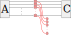
\includegraphics[width=0.7\linewidth, draft=false]{qds/individual_attacks}
	\end{subfigure}
	\begin{subfigure}{\linewidth}
		\centering
		\caption{\label{fig:types_of_attack_collective}}	
		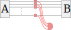
\includegraphics[width=0.7\linewidth, draft=false]{qds/collective_attacks}
	\end{subfigure}
	\begin{subfigure}{\linewidth}
		\centering
		\caption{\label{fig:types_of_attack_coherent}}	
		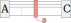
\includegraphics[width=0.7\linewidth, draft=false]{qds/coherent_attacks}
	\end{subfigure}
\caption{\label{fig:types_of_attack} Taxonomy of different eavesdropping attack strategies \cite{Lutkenhaus2004}. Black arrows denote quantum signal states distributed from Alice to Charlie. Red items belong to Bob. (a) Individual attack. Bob inserts separate probes (red boxes) into state distribution and performs measurement on each system individually. (b) Collective attack. Bob inserts separate probes into state distribution and stores his states until the end of signal distribution. He may then perform a measurement on his entire system. (c) Coherent attack. Bob interacts with all signals at the same time and he can perform a measurement on a single, global, probe. Attack (a) cannot introduce correlations between signals. Attack (b) may introduce classical correlations, and attack (c) may introduce any correlations between signals.}
\end{figure}

In this section we will focus on individual and collective forging attacks. Full security against coherent quantum attacks in the CV QKD literature has only been proven for the simpler case of coherent states modulated with a Gaussian distribution \cite{Lodewyck2007, Leverrier2010c, Pirandola2008, Leverrier2015, Laudenbach2017, Furrer2012}, and a full security proof remains elusive for a discrete modulation. There has been some recent success in applying convex optimization methods to the problem \cite{Ghorai2019, Lin2019}, but these proofs rely on an assumption about the Gaussianity of the discretely modulated alphabet \cite{Leverrier2009} which is only strictly valid in the limit $\alpha \rightarrow 0$. In keeping with recent trends in the QKD literature for discretely modulated coherent states without the assumption of Gaussianity \cite{Papanastasiou2018},  we will focus on bounding the attack strength of individual attacks, and then assume the i.i.d. criterion \cite{Leverrier2017, Laudenbach2017} in order to reach security against collective attacks. 


In particular, we will study both a beamsplitter attack and an entangling cloner attack for our protocol \cite{Grosshans2002, Grosshans2003}. In both of these attacks, Bob will replace the quantum distribution channel with a beamsplitter intended to mimic the effect of the channel on Charlie's measurement. Since Bob chooses his beamsplitter, he can do so without alerting Alice and Charlie to his presence, and so all channel loss must be attributed to Bob. Bob will either leave the second beamplitter input port empty, or he will mimic channel thermal noise by injecting there a thermal state Eq.~\ref{eqn:intro_thermal}, or one arm of his entangled two-mode squeezed vacuum state Eq.~\ref{eqn:intro_tmsv}. This so-called ``entangling cloner'' attack allows Bob to gain additional information which is stored in the correlations between his two modes. This is known to be a dishonest player's optimal attack strategy in asymptotic QKD with Gaussian-modulated coherent states \cite{Lodewyck2007, Laudenbach2017}, while the optimal attack strategy against discrete-modulated QKD remains an open question. However, we conjecture that entangling cloner should be optimal in the Gaussian limit $\alpha \rightarrow 0$, and close to optimal for the small amplitudes $\alpha$ considered in this thesis. Certainly, performing an entangling-cloner attack on each signal state as it passes will be physically demanding for Bob.

\subsection{Beamsplitter attack}

\begin{figure}[htp]
\captionsetup{width=0.8\linewidth}
\centering
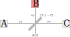
\includegraphics[draft=False,width=0.8\linewidth]{qds/BS0}
\caption{\label{fig:bs0_attack} Attack BS$0$. Bob replaces the channel with a lossless channel, plus a beamsplitter. By inputting vacuum $\dyad{0}$ into the beamsplitter, Bob mimics channel loss while imposing zero excess noise.}
\end{figure}

In its canonical form, the beamsplitter attack, Fig.~\ref{fig:bs0_attack}, allows Bob to replace a lossy channel, transmission $T$, with a corresponding lossless channel and beamsplitter. Bob inputs vacuum $\ket{0}$ into the unused input port. Bob receives his quantum system $\rho_B$ from the reflected output port, and from $\rho_B$ he will attempt to gain information about Charlie's measurement outcomes. Crucially, to honest players Alice and Charlie this attack is indistinguishable from simply having a lossy transmission channel, and so in analysis all channel loss must be attributed to the action of the dishonest Bob.  This attack cannot model any channel thermal noise, which should therefore be ignored in the analysis. A realistic channel will, however, impose noise onto Charlie's measurement outcomes, and later we describe some modificaions to the beamsplitter attack to include this.


\subsubsection{BS$0$: $\xi = 0$}\label{sec:qds_bs0}
Attack BS$0$ is depicted in Fig.~\ref{fig:bs0_attack}. This attack is the canonical beamsplitter attack, in which Bob will replace the channel with a lossless channel plus a beamsplitter. Crucially, the beamsplitter is chosen so that it mimics the channel exactly, and honest players should be unable to tell whether an attack has taken place. In a run of the protocol, therefore, all channel loss is attributed to dishonest Bob.


Consider a single input coherent state $\dyad{\alpha_k}$, with the $\alpha_k$ chosen uniformly at random from the QPSK alphabet ($k = 0,1,2,3$). Bob's attack effectively inputs the vacuum state $\dyad{0}$ into the second input port of the beamsplitter. We will calculate the Holevo information $\chi$, Eq.~\ref{eqn:intro_holevo}, of Bob's state conditioned on Charlie receiving a particular eliminated signature element after his heterodyne measurement.

Using beamsplitter relation Eq.~\ref{eqn:intro_beamsplitter} (c.f. Appendix~\ref{appendix:crypto_numerical_methods}), we see that a beamsplitter with transmission $T$ enacts the following transformation on the input state:
\begin{equation}\label{eqn:qds_coherent_state_beamsplitter}
\dyad{\alpha_k}_A \otimes \dyad{0}_B \rightarrow \dyad{\sqrt{T} \alpha_k}_C \otimes \dyad{\sqrt{1-T}\alpha_k}_{B}.
\end{equation}
So Charlie holds the state $\dyad*{\sqrt{T}\alpha_k}$, while Bob holds $\dyad*{\sqrt{1-T}\alpha_k}$. When the $\alpha_k$ is chosen uniformly at random, we must mix over the alphabet and so the mixed two-mode output state is
\begin{align}\label{eqn:qds_after_channel}
\left(\frac{1}{4}\sum_{\alpha_k} \dyad{\alpha_k}_A\right) &\otimes \dyad{0}_B \rightarrow \notag \\
&\frac{1}{4}\sum_{\alpha_k} \left(\dyad{\sqrt{T}\alpha_k}_C \otimes \dyad{\sqrt{1-T}\alpha_k}_B\right).
\end{align}

\noindent Charlie heterodynes on his mode and receives outcomes $\left(q_{\text{out}, C}, p_{\text{out}, C} \right)$. We write $z_C = q_{\text{out}, C} + i p_{\text{out}, C}$, and so Bob now holds
\begin{equation}\label{eqn:qds_bob_conditional_state}
\rho_{\left. B \given z_C \right.} = \frac{1}{4}\frac{1}{\text{P}\left(z_C\right)}\sum_{\alpha_k} \text{P}\left(z_C \given \alpha_k, T\right) \times \dyad{\sqrt{1-T}\alpha_k}_B.
\end{equation}
Here $\text{P}\left(z_C \given \alpha_k, T\right) = \left| \langle z_C | \sqrt{T}\alpha_k\rangle \right|^2$ corresponds to the probability that Charlie measures $z_C$ on his mode given that he received state $\dyad*{\sqrt{T}\alpha_k}$, while $\text{P}\left(z_C\right) = \sum_{\alpha_k} \text{P}\left(z_C | \alpha_k, T\right)$ corresponds to the total unconditional probability that he measures $z_C$.

Recall that the eliminated signature element held by Charlie is determined entirely by his heterodyne outcome $z_C$, Fig.~\ref{fig:qds_elimsig2}. Since Holevo information $\chi$ is defined in terms of Charlie's eliminated signature element rather than heterodyne measurement outcome, and since many outcomes $z_C$ will return the same eliminated signature element, we must now mix $\rho_{\left. B \given z_C \right.}$ over entire quadrants in phase-space.

\begin{figure}[htp]
\captionsetup{width=0.8\linewidth}
\centering

\includegraphics[draft=false, width=0.98\linewidth]{qds/elimsig2}
\caption{\label{fig:qds_elimsig2} Multiple heterodyne outcomes give rise to the same eliminated signature element. (a) A particular eliminated signature element. (b) All possible heterodyne outcomes consistent with (a).}
\end{figure}



Let us use the notation for eliminated signature elements from Tab.~\ref{tab:elimsig}, and consider the first eliminated signature element $e_1$. We mix $\rho_{\left. B \given z_C \right.}$ over all outcomes $z_C$ which are consistent with $e_1$, i.e. $\qout > 0$ and $\pout > 0$:

\begin{equation}\label{eqn:qds_aposterioristate}
\rho_{\left. B \given e_1\right.} = \frac{1}{\mathcal{N}\left(e_1\right)} \int\limits_{\qout>0, \pout>0} \Diff2 z_C \; \text{P}\left(z_C\right) \; \rho_{\left. B \given  z_C\right.},
\end{equation}
with the normalization factor\footnote{Clearly the normalization factor $\mathcal{N}$ as defined in Eq.~\ref{eqn:qds_aposterioristate_normalization} is equal to $1/4$ for each $e_1, e_2, e_3, e_4$. We explicitly show the general form for Eq.~\ref{eqn:qds_aposterioristate_normalization} here for completeness, though, as it will become important in Sec.~\ref{sec:qds_postselection} when we discuss postselection on measurement outcomes, and in Ch.~\ref{chapter:aqc} when assumptions about uniform sending probabilities are relaxed.} defined as
\begin{equation}\label{eqn:qds_aposterioristate_normalization}
\mathcal{N}\left(e_1\right) = \int\limits_{\qout>0, \pout>0} \Diff2 z_C \; \text{P}\left(z_C\right).
\end{equation}

\noindent The conditional state $\rho_{\left. B\given e_1\right.}$ is the quantum state held by Bob when Charlie has received eliminated signature element $e_1$. Bob's states conditioned on eliminated signature elements $e_2, e_3, e_4$ are calculated likewise by varying the limits of integration.

Bob's \emph{a posteriori} entropy, in terms of von Neumann entropy $S$, reads
\begin{equation}
S_{\text{aposteriori}} = \sum_{e_k} \text{P}\left(e_k\right) S\left(\rho_{\left. B \given e_k\right.}\right).
\end{equation}
In this chapter we are working in the ideal case where each eliminated signature element is equally likely, and where the entropies of each of the $\rho_{\left. B \given e_k\right.}$ are equal, and so we may simply write Bob's \emph{a posteriori} entropy as

\begin{equation}\label{eqn:aposteriori_entropy}
S_{\text{aposteriori}} = S\left(\rho_{\left. B \given e_1\right.}\right).
\end{equation}

\noindent Bob's \emph{a priori} state is given by
\begin{equation}\label{eqn:qds_aprioristate}
\rho_{\text{apriori}} = \sum_{e_k} \text{P}\left(e_k\right) \rho_{\left. B \given e_k\right.}
\end{equation}
and the corresponding \emph{a priori} entropy is simply $S\left(\rho_{\text{apriori}}\right)$. Finally, using the definiition of Holevo information, Eq.~\ref{eqn:intro_holevo},
\begin{equation}\label{eqn:qds_deriv_holevo}
\chi = S_{\text{apriori}} - S_{\text{aposteriori}}.
\end{equation}
We calculate and plot $\chi$ under attack BS$0$ in Fig.~\ref{fig:qds_holevo_comparisons}. 

\subsubsection{BS$1$: $\xi > 0$}\label{sec:qds_bs1}
\begin{figure}[htp]
\centering
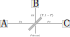
\includegraphics[draft=False, width=0.8\linewidth]{qds/BS1}
\caption{\label{fig:bs1_attack} Attack BS$1$. The beamsplitter mimics channel loss, while mixing with thermal state $\rho_{\text{thermal}}$ introduces excess noise into Charlie's outcome.}
\end{figure}
Next, let us consider a modification to attack BS$0$ which will allow us to model lossy channels which also induce excess noise in Charlie's measurement outcomes. In the first modification, denoted BS$1$ and displayed in Fig.~\ref{fig:bs1_attack}, Bob inputs a thermal state $\rho_{\text{thermal}}$, Eq.~\ref{eqn:intro_thermal}, into the second input port of the beamsplitter. This will induce excess noise $\xi > 0$ in Charlie's measurement outcomes consistent with the thermal channel noise,
where we define the excess noise in Charlie's $q$ quadrature, when coherent state $\ket{\alpha_k}$ was sent, as
\begin{equation}
\xi_q = \text{Var}\left(\qout \given \alpha_k\right) - \frac{1}{2},
\end{equation}
and similarly for $p$ quadrature. In other words, the excess noise in the $q$ quadrature is defined as the quadrature variance above the vacuum variance, and similarly for $p$. The total excess noise $\xi$ is then taken to be
\begin{equation}
\xi = \max \left\{ \xi_q, \xi_p\right\},
\end{equation}
and should be attributed to the action of dishonest Bob. We will calculate Bob's Holevo information under this attack.

We wish to mix a coherent state $\rho_{\alpha_k} = \dyad{\alpha_k}$ and a thermal state $\rho_{\text{thermal}}$ on a beamsplitter with transmission $T$. In Fock basis our states take the following form:

\begin{align}
&\rho_{\alpha_k} = e^{-\left|\alpha_k\right|^2} \sum_{n, m=0}^{\infty} \frac{\alpha_k^n \alpha_k^{* m}}{\sqrt{n! m!}} \dyad{n}{m} \notag \\
&\rho_{\text{thermal}} = \left(1 - e^{-\tilde{\beta}}\right) \sum_{p=0}^\infty e^{- p \tilde{\beta}}\dyad{p} \qq{with} \tilde{\beta} = \log_e\left(\frac{1}{\bar{n}} +1\right)
\end{align}

\noindent where $\alpha_k^{*}$ denotes the complex conjugate of $\alpha_k$. The input state into the beamsplitter is
\begin{equation}\label{eqn:qds_bs1_input_state}
\rho_{\text{input}} = \rho_{\alpha_k} \otimes \rho_{\text{thermal}}.
\end{equation}

\noindent Enacting beamsplitter relation Eq.~\ref{eqn:intro_beamsplitter_fock} on $\rho_{\text{input}}$, and heterodyning on Charlie's mode, we arrive at Bob's conditional output state $\rho_{\left. B \given z_C \right.}$. The state is displayed in full in Eq.~\ref{eqn:appendix_bs1_state}, Appendix.~\ref{appendix:bs1}.



Now, to reach the \emph{a posteriori} state under this attack we will integrate this $\rho_{\left. B \given z_C \right.}$ over all $z_C \in \mathbb{C}$ consistent with a particular eliminated signature element. Mathematically, this corresponds to simply integrating scalar terms involving $z_C$ in Eq.~\ref{eqn:appendix_bs1_state}, noting that the integration operation commutes with the rest of the state. Writing $z = z_C$ for convenience, the required integration is

\begin{equation}
\text{I}_{\text{BS}1} = \int\limits_{\qout>0, \pout>0} \Diff2 c \; z^k z^{* l} e^{ - \left| z \right|^2}
\end{equation}

\noindent where $k, l = 0, 1, 2, \dots$.

The integration is best performed in polar coordinates since the radial and angular integrals separate. We find
\begin{equation}\label{eqn:qds_bs1_deriv_3}
\text{I}_{\text{BS}1} =
\begin{cases}
\frac{\pi}{4} \Gamma\left(k+1\right) & \text{if } k = l; \\
\frac{-i}{k-l}\left(-1 + e^{i \frac{\pi}{2}\left(k-l\right)}\right)\frac{1}{2}\Gamma\left(\frac{1}{2}\left(k + l + 2\right) \right) & \text{if } k \ne l
\end{cases}
\end{equation}
with $\Gamma$ the gamma function \cite{mathworld_gamma}. Indeed, the radial component of the integrand of Eq.~\ref{eqn:qds_bs1_deriv_3} is a standard integral for $\Gamma$. The final \emph{a posteriori} state is now accessible by substituting Eq.~\ref{eqn:qds_bs1_deriv_3} into Eq.~\ref{eqn:appendix_bs1_state}.

The \emph{a priori} state is calculated likewise, but the limits of integration should be extended to the entire complex plane. In this case,
\begin{equation}\label{eqn:qds_bs1_deriv_4}
\int\limits_{\mathbb{C}} \Diff2 c \; e^{-\left|z\right|^2}z^k z^{* l} = \pi \Gamma\left(k+1\right)
\end{equation}
since the polar integral forces $k=l$. The Holevo information may now be calculated in the same way as Sec.~\ref{sec:qds_bs0} by the difference of \emph{a priori} and \emph{a posteriori} entropies, and we compare Holevo information under different attacks in Fig.~\ref{fig:qds_holevo_comparisons}.
%\MT{where do I want to talk about truncating matrices and numerical methods?}



\subsection{Entangling-cloner attack}\label{sec:qds_ec}
\begin{figure}[htp]
\captionsetup{width=0.8\linewidth}
\centering
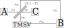
\includegraphics[draft=False, width=0.8\linewidth]{qds/EC}
\caption{\label{fig:ec_attack} EC attack. Locally, one mode of the TMSV looks like $\rho_{\text{thermal}}$ and so allows channel excess noise to be emulated. Bob can exploit correlations in noise between his two mode output state $\rho_{B_1^\prime, B_2}$ to gain additional information.}
\end{figure}
The entangling cloner attack \cite{Grosshans2002, Grosshans2003}, depicted in Fig.~\ref{fig:ec_attack}, is ideally suited to consistently incorporate the presence of excess noise $\xi$, and we shall see that it is a much more powerful attack than any of the beamsplitter attacks considered above. The entangling cloner attack, which we shall denote EC, may be viewed as a natural extension of attack BS$1$.  %EC is known to be the optimal collective attack for

Instead of inputting a thermal state into the beamsplitter's fourth port, Bob will input one arm of his entangled two-mode squeezed vacuum (TMSV) state, Eq.~\ref{eqn:intro_tmsv}. The mode which Bob inputs into the channel is locally indistinguishable from $\rho_{\text{thermal}}$, and so honest players are unable to distinguish between BS$1$, BS$2$ and EC.

%The $EC$ attack has a long history, and is known to be the optimal collective attack for gPSK QKD \MT{cite a bunch of stuff}. Since our QPSK alphabet is non-Gaussian we make no claims as to $EC$'s optimality, though we conjecture that $EC$ will be optimal as $\alpha \rightarrow 0$, and close to optimal for $\alpha << 1$. The status of optimal attacks on QDS is an open one and should be the subject of further exploration. The question about optimal attacks on QKD with discrete modulated coherent states is also open, despite a long history of activity on these protocols. In any case, the $EC$ attack is very difficult to perform with today's technology, and so a protocol with security against $EC$ (or even $BSx$) attacks should be expected to be practically secure for a long time.

%\MT{Talk somewhere about where the extra power in the EC attack comes from - we allow Bob to exploit also the correlations between his two modes. Also have some figures of histograms of this attack}

Let us analyse the EC attack. Alice creates the coherent state $\dyad*{\alpha_k}$, while Bob generates
\begin{equation}\label{eqn:qds_ec_tmsv}
\tmsv = \frac{1}{\cosh^2 \zeta}  \sum_{n, m=0}^\infty \left(\tanh\zeta\right)^{n+m} \dyad{n, n}{m, m}.
\end{equation}

\noindent Let us write the three-mode input state to the channel as

\begin{align}
\rho_{\text{input}} &= \frac{e^{-\left|\alpha_k\right|^2}}{\cosh^2 \zeta} \sum_{n_1, m_1=0}^\infty \sum_{n_2, m_2=0}^{\infty} \frac{\alpha_k^{n_1} \overline{\alpha_k}^{m_1}}{\sqrt{n_1! m_1!}} \left(\tanh\zeta\right)^{n_2 + m_2} \notag \\
&\times \bigg[\dyad{n_1, n_2}{m_1, m_2}\bigg] \otimes \dyad{n_2}{m_2},
\end{align}

\noindent where we have explicitly separated in square brackets the two modes which will interfere on the beamsplitter.

The beamsplitter mixes $\dyad{n_1, n_2}{m_1, m_2}$ via Eq.~\ref{eqn:intro_beamsplitter}, and gives an entangled three-mode state at the output. Charlie heterodynes on his mode and receives outcome $z_C$, and we arrive at Bob's conditional two-mode output state $\rho_{\left. B \given z_C\right.}$, which we display fully in Eq.~\ref{eqn:appendix_ec_state}, Appendix.~\ref{appendix:ec_state}. %A histogram of Bob's conditional two-mode state is displayed in Fig.~\ref{fig:appendix_qds_ec_histogram} where we see that his state depends heavily on Charlie's outcome $c$.  TODO: Put this sentence and the figure in the appendix

Once again the state is readily integrated in $z_C$, either over the entire complex plane or a single quadrant, and we may simply substitute Eqs.~\ref{eqn:qds_bs1_deriv_3},~\ref{eqn:qds_bs1_deriv_4} into Eq.~\ref{eqn:appendix_ec_state} to reach the \emph{a posteriori} and \emph{a priori} states, respectively.

The \emph{a priori} state is automatically normalized by virtue of the integration over $\mathbb{C}$, while the \emph{a posteriori} state is normalized by multiplying by $\mathcal{N}\left(e_1 \given \xi \right)$, defined as 

\begin{equation}
\mathcal{N}\left(e_1 \given \xi\right) = \int\limits_{\qout>0, \pout>0} \Diff2 c \; \text{P}\left(z_C \given \xi \right).
\end{equation}
where we have included excess noise $\xi$ in our probability, as in Appendix.~\ref{appendix:noisy_perr}. The performance of this attack is analysed in Fig.~\ref{fig:qds_holevo_comparisons}.


\subsection{Comparison of attacks}

We compare attacks BS$0$, BS$1$ and EC in Fig.~\ref{fig:qds_holevo_comparisons} as amplitude $\alpha$ and channel transmission $T$ are varied. We observe that for all $\alpha, T$ and for all channel thermal photon numbers $\bar{n}$ the EC attack performs best, while attack BS$1$ performs worse than even attack BS$0$ where no excess noise is considered. Under EC, Bob is permitted to exploit correlations between his two modes, and the $\bar{n}$ restricts the level of entanglement between his modes. Larger $\bar{n}$ means greater entanglement, and so we should expect that as $\bar{n}$ increases Bob gains more information. However, under BS$1$ Bob is not permitted to use these correlations, and so his outcomes and Charlie's outcomes are both noisy. The added noise reduces Bob's information without providing him the advantage of EC. 

The thermal photon number $\bar{n}$ is related to the inverse temperature of the input thermal state in BS$1$ as \cite{Leonhardt2010}
\begin{equation}
\beta = \log_e\left(\frac{1}{\bar{n}} + 1\right),
\end{equation}
while $\bar{n}$ is related to the squeezing parameter $\zeta$ of the input TMSV state in EC as \cite{Leonhardt2010}
\begin{equation}
\zeta = \text{Sinh}^{-1}\left(\sqrt{\bar{n}}\right).
\end{equation}

\begin{figure}[htp]
\captionsetup{width=0.8\linewidth}
\centering
	\begin{subfigure}{0.7\linewidth}
		\centering
		\caption{\label{fig:qds_holevo_comparisons_varalpha}}
		\includegraphics[draft=false, width=\linewidth]{qds/holevo_comparisons_varalpha}
	\end{subfigure}
	\begin{subfigure}{0.7\linewidth}
		\centering
		\caption{\label{fig:qds_holevo_comparisons_varT}}
		\includegraphics[draft=false, width=\linewidth]{qds/holevo_comparisons_varT}	
	\end{subfigure}
	\caption{\label{fig:qds_holevo_comparisons} Comparison of Holevo information $\chi$ under attacks BS$0$ (black), BS$1$ (orange) and EC (red). BS$0$ has no excess noise in the channel which corresponds to channel thermal photon number $\bar{n} = 0$. BS$1$ and EC both include excess noise, with $\bar{n} = 0.01$ (solid red/orange lines) and $\bar{n} = 0.02$ (dashed red/orange lines). (a) Increasing amplitude $\alpha$ of the QPSK alphabet leads to larger Holevo information for dishonest Bob. Honest players should therefore choose small $\alpha$. (b) At $T=0$ and $T=1$ Bob gains no information about Charlies outcomes. In both (a) and (b), we see that EC attack gives Bob much more information than BS$0$, while BS$1$ performs worse.}
\end{figure}

Since under attack BS$1$ Bob performs worse than BS$0$, we are led to consider an attack which can be considered mid-way between the power of BS$0$ and EC. We modify the attack by imposing that the channel excess noise should \emph{only} affect honest players. That is, the presence of $\xi$ causes $\perr$ to increase, but Holevo information and therefore $\pe$ should both be unaffected. We call this attack BS$2$. While strictly this attack is physically inconsistent, and therefore impossible for Bob to perform, it is more pessimistic for honest players than either BS$0$ or BS$1$ and so the security bounds it gives are also safe bounds on both of those attacks. Indeed, since an analytic expression for Bob's states under attack BS$0$ is readily attainable without resort to the numerical methods required for BS$1$ (Appendix~\ref{appendix:crypto_numerical_methods}), in some circumstances it may even be computationally preferable to assume attack BS$2$. The Holevo information is given by using Eqs.~\ref{eqn:qds_aposterioristate} and \ref{eqn:qds_aprioristate} in the usual way, while $\perr$ is given in Appendix~\ref{appendix:noisy_perr}.


\clearpage
\section{Signature length $L$}\label{sec:qds_siglength}
%\MT{better segue}
We have proven protocol security against both repudiation (Sec.~\ref{sec:qds_security_repudiation}) and forgery (Sec.~\ref{sec:qds_security_forgery}). and we have shown that our QDS protocol is robust (Sec.~\ref{sec:qds_security_robustness}). Additionally, we have demonstrated how a forging Bob's probability $\pe$ to introduce a mismatch into his signature is related to the Holevo information $\chi$ of his quantum system (Sec.~\ref{sec:qds_bounding_pe}) and have explicitly analysed several attacks which he may perform which mimic different channel conditions (Sec.~\ref{sec:qds_attack_analysis}). We are now in a position to calculate the total probability that our QDS protocol fails to meet the security requirements outlined in List.~\ref{list:qds_requirements}. We shall see that the total failure probability decays exponentially, and so our protocol is secure.

Let us define $\varepsilon_{\text{fail}}$ as the total probability that our protocol fails, either by allowing a repudiation or forging attack, or by aborting when all players behaved honestly. To gain a figure of merit we assume that the protocol is equally likely to fail in any of these ways, and so we set
\begin{equation}\label{eqn:qds_efail_deriv}
\varepsilon_{\text{fail}} = \varepsilon_{\text{honest abort}} = \varepsilon_{\text{repudiation}} = \varepsilon_{\text{forgery}},
\end{equation}
though we note that alternative combinations may be easily considered. Let us eliminate the free parameters $s_B, s_C$ by equating the arguments of Eqs.~\ref{eqn:erep},~\ref{eqn:ehonabort}, \ref{eqn:eforg}:
\begin{equation}
\left(\pe - s_C\right)^2  = \frac{1}{4}\left(s_C - s_B\right)^2 = \left(s_B - \perr\right)^2,
\end{equation}
from which we may derive
\begin{equation}\label{eqn:qds_sbsc}
s_B = \frac{3}{4} \perr + \frac{1}{4}\pe \qq{and} s_C = \frac{1}{4}\perr + \frac{3}{4}\pe,
\end{equation}
as our choices of security thresholds. Notice that since $\perr \le \pe$, Eq.~\ref{eqn:qds_sbsc} automatically fulfils the requirement that $s_B \le s_C$. The overall probability of failure Eq.~\ref{eqn:qds_efail_deriv} therefore becomes

\begin{equation}\label{eqn:efail}
\varepsilon_{\text{fail}} \le 2 \text{exp}\left( - \left[\pe - \perr\right]^2 \frac{L}{16}\right).
\end{equation}

\noindent This probability $\varepsilon_{\text{fail}}$ decays exponentially in $L$, and so provided that $\perr$ and $\pe$ are known, and $\pe - \perr \ge 0$, any security level $\varepsilon_{\text{fail}} > 0 $ may be reached by varying signature length $L$. In keeping with the recent works Refs.~\cite{Collins2014, Croal2016, Donaldson2016, Amiri2016} in this Thesis we will take $\varepsilon_{\text{fail}} = 0.01\%$. Equation~\ref{eqn:efail} may then be solved for the signature length. We take $L$ as the main figure of merit\footnote{Analogously to the key rate in QKD.} for a QDS protocol, and analyse the performance of our protocol in Sec.~\ref{sec:qds_protocol_performance}.



\section{Postselection}\label{sec:qds_postselection}
In the context of QKD it has been known for some time that a postselection of measurement outcomes, in which measurement outcomes unfavourable to honest players are discarded, will improve the key rates in the presence of excess noise. Postselection is even a requirement to distill a key below $T \le 1/2$ in the direct reconciliation regime \cite{Silberhorn2002}. We are thus motivated to apply postselection to our QDS protocol in order to allow a message to be securely signed over a larger range of channel parameters, and we shall see that it can reduce the necessary $L$. The results of this section will be especially useful in Ch.~\ref{chapter:aqc} where -- as for direct reconciliation QKD -- we shall see that postselection is a necessity for some QDS protocols.

For now, we will apply postselection to the protocol outlined in this chapter. To apply the postselection technique, recipients Bob and Charlie will simply disregard unfavourable measurement outcomes, i.e. outcomes for which a dishonest player is deemed to have too much knowledge, or for which the probability of honest mismatch is too high.

We define a region $\rps \in \mathbb{C}$, Fig.~\ref{fig:rps}. Honest recipients will only accept measurement outcomes $\left(\qout, \pout\right)$ with $c := \qout + i \pout \in \mathbb{C}\setminus\rps$. We may then vary $\rps$ in order to increase the range of channel parameters for which the QDS protocol is secure, and to minimize signature length $L$.

\begin{figure}[htp]
\captionsetup{width=0.8\linewidth}
\centering
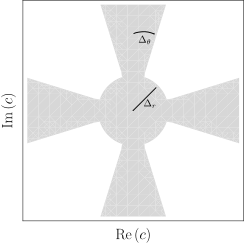
\includegraphics[draft=false, width=0.7\linewidth]{qds/rps2}
\caption{\label{fig:rps} The postselection region $\rps$, gray, is parametrized by $\Delta_r, \Delta_\theta$ in polar coordinates. Participants will only accept measurement outcomes $c \in \mathbb{C} \setminus \rps$. }
\end{figure}

Our chosen $\rps$ is parametrized by two variables $\Delta_r, \Delta_\theta$ in polar coordinates, Fig.~\ref{fig:rps}. This is the same postselection region which was considered in the recent work Ref.~\cite{Lin2019}, but if desired more general regions may be readily considered. We make no claims as to the optimality of our choice of the shape $\rps$, though once the form of $\rps$ is set we may optimize over $\Delta_r$ and $\Delta_\theta$ to improve protocol security.

The crucial quantity which controls the security of our QDS protocol is $g_{\text{sec}} := \pe - \perr$, which describes how much more likely a dishonest player is to induce a mismatch than an honest player. We saw in Sec.~\ref{sec:qds_siglength} that our QDS protocol is secure provided that $g_{\text{sec}} > 0$, and that the signature length $L$ required to sign to a given level of security $\varepsilon_{\text{fail}}$ is directly controlled by $g_{\text{sec}}$. We therefore must consider how postselection affects $g_{\text{sec}}$. 

Let us begin with the effect of postselection on $\perr = \perr\left(\Delta_r, \Delta_\theta\right)$. %\MT{I don't want to talk yet about calculating $\perr$ from data - that should wait until the agile chapter.} 
Recall that when Alice sends state $\ket{\alpha}$ through a lossy but noiseless channel, transmission $T$, Charlie receives $c \in \mathbb{C}$ with probability

\begin{equation}
\text{P}\left(c \given \alpha, T\right) = \frac{1}{\pi} \exp\left( - \left| c - \sqrt{T}\alpha\right|^2\right).
\end{equation}

\noindent Thus the probability of eliminating the state $\ket{\alpha}$ when no postselection is used is, in polar coordinates,
\begin{align}\label{eqn:perrps_deriv_nops}
\perr &= \int\limits_{r=0}^\infty \mathrm{d}r \; r \int\limits_{\theta = \pi/2}^{3 \pi/2} \mathrm{d}\theta \; \text{P}\left(r e^{i \theta} \given \alpha, T\right) \notag \\
%
&= \frac{1}{2}\erfc\left(\sqrt{\frac{T}{2}}\left|\alpha\right|\right).
\end{align}

\noindent When the postselection technique is used we must change the limits of integration, so the mismatch probability becomes

\begin{align}\label{eqn:perrps_deriv_2}
\perr\left(\Delta_r, \Delta_\theta\right) %= \frac{1}{\mathcal{N}} \int\limits_{\left.x \in \mathbb{C} \setminus \rps \given \text{Re}\left(x\right) < 0\right. } \Diff2 x \; \text{P}\left(x \given \alpha, T\right) \notag \\
= \frac{1}{\mathcal{N}} \int\limits_{\Delta_r}^{\infty} \mathrm{d}r \; r &\left[ \; \int\limits_{ \pi/2 + \Delta_\theta}^{\pi - \Delta_\theta} \mathrm{d}\theta \; \text{P}\left(r e^{i \theta} \given \alpha, T\right) \right. \notag \\
%
 &+ \left. \int\limits_{3 \pi/2 - \Delta_\theta}^{\pi + \Delta_\theta} \mathrm{d}\theta \; \text{P}\left(r e^{i \theta} \given \alpha, T\right) \right],
\end{align}


\noindent where we effectively have the same integrals as Eq.~\ref{eqn:perrps_deriv_nops} restricted by $\rps$. The normalization probability $\mathcal{N}$ is the probability that Charlie will accept his measurement outcome, which is calculated by extending the integration in Eq.~\ref{eqn:perrps_deriv_2} to the entire $\mathbb{C} \setminus \rps$

\begin{equation}\label{eqn:qds_perrps_normalization}
\mathcal{N} = \int\limits_{\mathbb{C} \setminus \rps} \Diff2 c \; \text{P}\left(c \given \alpha, T, \xi \right).
\end{equation}

\noindent The calculation of $\perrps$ follows identically to Eq.~\ref{eqn:perrps_deriv_2} when excess noise $\xi$ is included, simply using the requisite formula (Appendix~\ref{appendix:noisy_perr}) and performing the integrations as Eq.~\ref{eqn:perrps_deriv_2}.


Since a dishonest player's declaration will depend on an honest player's heterodyne outcome, the probability $\pe$ must also vary with $\rps$. We will calculate the effect of $\rps$ on Holevo information $\chi$, from which the probability $\pe$ is calculated via Eq.~\ref{eqn:qds_hpe} as normal.

%Let Bob's $j^{\text{th}}$ \emph{a posteriori} state be $\rho_{B | e_k}^j$, which is conditioned on Charlie holding eliminated signature element $e_k$. 
Assume that Bob has performed any one of the attacks examined in Sec.~\ref{sec:qds_attack_analysis}, and let Bob's state after Charlie's heterodyne measurement be denoted $\rho_{\left. B \given c\right.}^j$. Again, since Charlie's eliminated signature element is entirely determined by the quadrant in which $c$ lies, the state $\rho_{\left. B \given  e_k\right.}^j$ is calculated by mixing $\rho_{\left.B \given c\right.}^j$ over an entire quadrant of phase-space, as in Eqs.~\ref{eqn:qds_aposterioristate},~\ref{eqn:qds_bs1_deriv_3}, Tab.~\ref{tab:elimsig}. We must therefore update these integrals to include the effect of $\rps$. For example,

\begin{align}\label{eqn:qdsps_aposteriori}
\rho_{\left.B \given e_1\right.}^j = \frac{1}{\mathcal{N}} \int \Diff2 c \; \rho_{\left. B \given c\right.}^j
%
=\frac{1}{\mathcal{N}} \int\limits_{\Delta_r}^\infty \mathrm{d}r\; r\int\limits_{\Delta_\theta}^{\pi/2 - \Delta_\theta} \mathrm{d}\theta \; \rho_{\left. B \given r e^{i \theta}\right.},
\end{align}

\noindent and similarly for $e_2, e_3, e_4$. The $\mathcal{N}$ is identical to that required for Eq.~\ref{eqn:perrps_deriv_2}, and Bob's $\emph{a priori}$ state is found by mixing Eq.~\ref{eqn:qdsps_aposteriori} over all quadrants. Probability $\pe\left(\Delta_r, \Delta_\theta\right)$ may now be calculated via Eq.~\ref{eqn:qds_hpe}. 

To actually perform the integration, we separate out terms involving $c$ in Bob's state %(see Secs.~\ref{sec:qds_bs0},~\ref{sec:qds_ec},~\ref{sec:appendix_bs1_state},~\ref{sec:appendix_ec_state}) , 
and so the integration becomes

\begin{equation}
\frac{1}{\mathcal{N}} \int\limits_{\Delta_r}^{\infty} \mathrm{d}r \; r \int\limits_{\Delta_\theta}^{\pi/2 - \Delta_\theta} \mathrm{d}\theta \; r^k r^l e^{-r^2} e^{i \theta \left(k - l\right)}.
\end{equation}

\noindent where we have used $c = r e^{i \theta}$. To perform the integration, it is helpful to perform the angular integral first, which readily integrates to a sum of exponentials when $k \ne l$, or to $\pi/2 - 2\Delta_\theta$ when $k=l$. The remaining radial term is

\begin{equation}\label{eqn:qds_perrps_radial_integration}
\int\limits_{\Delta_r}^\infty \mathrm{d}r \; r^{k + l + 1} e^{-r^2}
\end{equation}

\noindent which is the definition of an upper incomplete Gamma function \cite{Mathworld_Incomplete_Gamma}, which we denote as $\Gamma_\uparrow$. The radial integration Eq.~\ref{eqn:qds_perrps_radial_integration} is thus identically

\begin{equation}
\Gamma_{\uparrow}\left(\frac{1}{2}\left[2 + k + l\right], \Delta_r^2\right)  \forall k, l \ge 0
\end{equation}
which may be easily calculated.

We have now included the effects of $\rps$ on $g_{\text{sec}}$, and so the performance of the protocol under postselection may be analysed. In Fig.~\ref{fig:qds_gsec_varying_rps} we plot $g_{\text{sec}}$ varying $\rps$ for attacks BS$0$, BS$1$, and EC, and for different coherent state amplitude $\alpha$'s at $T=0.5$. We observe that when considering $g_{\text{sec}}$, it is advantageous to choose a large postselection region as this always allows $g_{\text{sec}}$ to increase. However we also observe that the effectiveness of postselection depends on our coherent state amplitude. For example, at $\alpha=0.2$ we see smaller increase in $g_{\text{sec}}$ as $\rps$ is increased, and there is almost no effect of postselection as $\Delta_\theta$ is varied under EC attack.


\begin{figure}[htp]
\captionsetup{width=0.8\linewidth}
\centering
	\begin{subfigure}{0.7\linewidth}
		\centering
		\caption{}
		\includegraphics[draft=false, width=\linewidth]{qds/rps_varying_gsec_1}
	\end{subfigure}
	\begin{subfigure}{0.7\linewidth}
		\centering
		\caption{}
		\includegraphics[draft=false, width=\linewidth]{qds/rps_varying_gsec_2}
	\end{subfigure}
\caption{\label{fig:qds_gsec_varying_rps} The efficacy of postselection depends strongly both on attack type and parameters $\alpha, T$. Solid: $\Delta_\theta = 0$. Dashed: $\Delta_\theta = 0.3$. Green: BS$0$. Orange: BS$1$.  Red: EC. (a) $\alpha = 0.5, T=0.5$ and (b) $\alpha = 0.2, T=0.5$. In both graphs attacks BS$1$ and EC have excess noise $\xi = 0.1\%$.  }
%Calculations/Cryptography/2020-02-11_gsec_varying_rps
%Technically, blue is BS0 and Green is BS2, but they are basically overlapping and I am trying to downplay attack BS2.
%This caption originally said that \xi=0.001% but I have changed it because I think it was wrong. TODO: check
\end{figure}


Let us turn now to examine our main figure of merit, the number of quantum states $L$ used in the protocol. Directly incorporating $g_{\text{sec}}\left(\Delta_r, \Delta_\theta\right)$ into Eq.~\ref{eqn:efail} will give an erroneous level of security, for the following reason. Our calculations in this section, culminating in $g_{\text{sec}}\left(\Delta_r, \Delta_\theta\right)$, correctly bound the number of states required to sign a message to security level $\varepsilon_{\text{fail}}$. However, this is not equivalent to the number of states which Alice has actually sent. 

For example under attack EC with $\alpha=0.5, T=0.5, \xi=0.1\%$, choosing $\Delta_r = 4.0 $ and $\Delta_\theta = 0.4 $ gives $g_{\text{sec}} = 0.1225 $. Substituting this into Eq.~\ref{eqn:efail} and solving for $L$ gives $L = 10560$. But in order to have that many states accepted at Charlie, Alice will actually need to have sent $7\times10^{10}$ coherent states in total, since Charlie will reject his measurement outcomes with probability $1 - \left(1.5\times10^{-7}\right)$, Eq.~\ref{eqn:qds_perrps_normalization}. It follows that $L$, as implicitly defined by Eq.~\ref{eqn:efail}, is actually a poor figure of merit to measure the resource-use of our protocol when postselection is used.

Instead, we will work in terms of $\tilde{L}$, which we define as the total number of states sent by Alice. This may be written as a rescaling of $L$ given by
\begin{equation}
L \mapsto \tilde{L} := \frac{L}{\mathcal{N}},
\end{equation}
with the normalization factor $\mathcal{N}$ interpreted sthe average probability that Charlie accepts a given state sent by Alice, Eq.~\ref{eqn:qds_perrps_normalization}.

We plot $\mathcal{N}$ in Fig.~\ref{fig:psnorm}, and figure of merit $\tilde{L}$ in Fig.~\ref{fig:qds_L_vs_deltar}. We observe that even though large $\Delta_\theta$ causes $g_{\text{sec}}$ to increase, Fig.~\ref{fig:qds_gsec_varying_rps}, it also causes an increase in $\tilde{L}$, owing to the quick decay of $\mathcal{N}$ with $\Delta_\theta$, Fig.~\ref{fig:psnorm}. We also may deduce from the graphs Fig.~\ref{fig:qds_L_vs_deltar} that there is an optimum $\Delta_r$ which minimizes $\tilde{L}$ and gives the best performance of our protocol.


\begin{figure}[htp]
\captionsetup{width=0.8\linewidth}
\centering
\begin{subfigure}{0.4\linewidth}
\includegraphics[draft=false, width=\linewidth]{qds/psnorm1}
\caption{}
\end{subfigure}
\begin{subfigure}{0.4\linewidth}
\includegraphics[draft=false, width=\linewidth]{qds/psnorm2}
\caption{}
\end{subfigure}
\caption{\label{fig:psnorm} Normalization factor $\mathcal{N}$ Eq.~\ref{eqn:qds_perrps_normalization} varies dramatically with postselection region $\rps$. (a) $\alpha=0.5, T=0.5$. (b) $\alpha=3.0, T=1.0$}
%images/qds/psnorm.nb
\end{figure}

\begin{figure}[htp]
\captionsetup{width=0.8\linewidth}
\centering
	\begin{subfigure}{0.7\linewidth}
		\centering
		\caption{}
		\includegraphics[draft=false, width=\linewidth]{qds/rps_varying_L_1}
	\end{subfigure}
	\begin{subfigure}{0.7\linewidth}
		\centering
		\caption{}
		\includegraphics[draft=false, width=\linewidth]{qds/rps_varying_L_2}
	\end{subfigure}
\caption{\label{fig:qds_L_vs_deltar} The key figure of merit, $\tilde{L}$, depends strongly on postselection region $\rps$. Solid: $\Delta_\theta=0$. Dashed: $\Delta_\theta = 0.3$. Green: BS$0$. Orange: BS$1$. Red: EC. (a) $\alpha = 0.5, T = 0.5$ and (b) $\alpha=0.2, T=0.5$. In both graphs attacks BS$1$ and EC have $\xi = 0.1 \%$. In all cases it is optimal to choose $\Delta_\theta = 0$}
%Calculations/Cryptography/2020-02-12_L_varying_rps.nb
\end{figure}

Since the figures of merit $\tilde{L}$ (with postselection)and $L$ (without postselection) qualitatively measure the same thing -- how many states must Alice send in order to sign a $1$~bit message -- they may be directly compared. For the remainder of this Thesis, then, we will not distinguish between $\tilde{L}$ and $L$. It should be understood that when postselection is used we are using the rescaled $\tilde{L}$, while when postselection is not use we are using $L$. Furthermore, since $\Delta_\theta > 0$ causes $\tilde{L}$ to increase we will take the optimal $\Delta_\theta=0$ always from now on, and only allow $\Delta_r$ to vary. It will be made clear in what follows whether the postselection technique has been used and the choice of $\Delta_r$.



%\clearpage
\section{Protocol performance}\label{sec:qds_protocol_performance}
Let us apply the analysis performed in the previous few sections and calculate our main figure of merit, the signature length $L$, under several different attacks. We plot the signature length $L$ required to sign a $1$~bit message under attacks BS$0$ (black) and EC (red) in Fig.~\ref{fig:qds_nonoptimal_L}, for several different $\alpha$. An entangling cloner attack with $\xi = 0.1\%$ has vastly increased signature length for $\alpha=0.2$ (dotted), while for larger $\alpha=0.5, 0.8$, entangling-cloner causes the signature length to by more modest amounts when compared to BS$0$. Note that in Fig.~\ref{fig:qds_nonoptimal_L} the transmissions $T$ at which the lines stop should be interpreted as being close to the smallest $T$ attainable before $L$ begins to diverge, and signing a message becomes impractical (in the case of BS$0$) or impossible (in the case of EC). 





\begin{figure}[htp]
\captionsetup{width=0.8\linewidth}
\centering
\includegraphics[width=0.7\linewidth, draft=false]{qds/QDSf_nonoptimal_L}
\caption{\label{fig:qds_nonoptimal_L} Signature lengths $L$ varying with channel transmission $T$ for attacks BS$0$ (black) and EC (red). Solid: $\alpha=0.5$. Dashed: $\alpha=0.8$. Dotted: $\alpha=0.2$. Entangling cloner attack has excess noise $\xi = 0.1\%$ at all T. A non-optimal choice of $\alpha$ can lead to much larger signature lengths. No postselection is used.}
\end{figure}


Even when attack BS$0$ is used and $\xi=0\%$, a sub-optimal choice of coherent state amplitude $\alpha$ can drastically worsen the performance of the protocol. To investigate optimal amplitudes, we plot the security parameter $g_{\text{sec}}$ varying with $\alpha$ under attack BS$0$ in Fig.~\ref{fig:qds_gsec_croal}. We observe that the optimal $\alpha$ decreases with increasing loss (smaller $T$). Intuitively, at $T=1.0$ Eve gains no information and so one should pick $\alpha \gg 1$ so as to minimize mismatch rate between honest players. 

We also compare our current protocol to a recent CV QDS protocol \cite{Croal2016} which did not allow for the presence of an eavesdropper on the quantum channels. The security parameter under Ref.~\cite{Croal2016} is displayed as red, dot-dashed lines in Fig.~\ref{fig:qds_gsec_croal} at $T=0.47$ (top) and $T=0.19$ (bottom). We see that for larger $T$, and almost all $\alpha$ at smaller $T$, our current protocol outperforms Ref.~\cite{Croal2016}, despite our relaxing the requirement of secure quantum channels. This surprising improvement in performance comes directly from the fact that in the current protocol, Alice distributes different signatures to each recipient, whereas in Ref.~\cite{Croal2016} she distributed identical signatures.

\begin{figure}[htp]
\captionsetup{width=0.8\linewidth}
\centering
\includegraphics[width=0.7\linewidth, draft=false]{qds/Thornton2019_croal_comparisons}
\caption{\label{fig:qds_gsec_croal} Security parameter $g_{\text{sec}}$ under attack BS$0$ as it varies with $\alpha$ for $T = 0.61$, $0.47$, $0.19$, $0.11$, $0.01$ (solid, black, top to bottom). The optimal $\alpha$ which should be chosen to maximize $g_{\text{sec}}$ (minimize L) decreases as $T$ decreases. Horizontal gridlines denote $\mathcal{O}\left(L\right)$ starting from $L \sim 10^5$ at $g_{\text{sec}} = 0.038$ (top), with $L$ increasing by a factor of $10$ at subsequent lower gridlines. Red, dot-dashed: $g_{\text{sec}}$ calculated via the protocol described in Ref.~\cite{Croal2016} for $T=0.19$ and $T=0.47$.}
\end{figure}

We optimize over $\alpha$ and postselection region $\Delta_r$ in Fig.~\ref{fig:qds_optimal_L}. The figure thus represents the smallest attainable $L$ for our protocol under attacks BS$0$ (solid, blue), BS$2$ (dashed, orange) and EC (solid, red). Attack BS$1$ gives smaller $L$ than even BS$0$, and so we do not show it. Even at the $T \sim 0.4$ corresponding to a fiber length $\sim 20$~km, the attainable $L$ are very modest at only $\mathcal{O}\left(10^5\right)$ under BS$0$ and $\mathcal{O}\left(10^6\right)$ for EC attacks. 


\begin{figure}[htp]
\captionsetup{width=0.8\linewidth}
\centering
\includegraphics[width=0.7\linewidth, draft=false]{qds/QDSf_optimal_L}
\caption{\label{fig:qds_optimal_L} Signature lengths under protocols BS$0$ (blue, solid), BS$2$ (orange, dashed) and EC (red, solid). At each point $L$ is optimized over $\alpha$ and postselection parameter $\Delta_r$. EC attack with $\xi = 0.1\%$.}
\end{figure}

Finally, in Appendix~\ref{appendix:qds_larger_alphabets} we extend the protocol discussed in this chapter to allow for larger alphabet sizes. These alphabets, which we denote as $N$PSK alphabets, consist of $N$ coherent states equally distributed around the origin of phase space. The case $N=4$ is equivalent to the QPSK alphabet which we have used until now. For $N$PSK alphabets with $N=2$, $N=4$, $N=6$, $N=8$ we plot their signature lengths optimized over $\alpha$ in Fig.~\ref{fig:qds_npsk_length_body}, and the required optimal $\alpha$'s are displayed in the inset. 

Surprisingly, although for larger alphabets the optimal $\alpha$ is decreased, the minimal $L$ is slightly increased. As has been found elsewhere \cite{Leverrier2011}, the biggest leap in behaviour should occur between $2 \rightarrow 4$, and indeed this is what we see\footnote{Noting that for the case $N=2$ we no longer need to think about an eliminated signature and we may simply consider optimal guessing probabilities.}. As $N$ increases, with $\alpha \ll 1$ we tend closer towards a Gaussian mixture of coherent states (c.f. Fig.~\ref{fig:intro_npsk}b). We may therefore reasonably expect the attack strategies BS$0$ and EC to become increasingly optimal in this Gaussian limit, which explains the slight increase in $L$ for larger alphabets.

\begin{figure}[htp]
\captionsetup{width=0.8\linewidth}
\centering
\includegraphics[width=0.7\linewidth, draft=false]{qds/appendix_npsk_length}
\caption{\label{fig:qds_npsk_length_body} Signature length $L$ under attack BS$0$. At each $T$, length $L$ has been optimized over amplitude $\left|\alpha\right|$ of the alphabet. We have considered $N$PSK alphabets with $N = 2$, $4$, $6$, $8$. Dot-dashed: $N=2$. Black, solid: $N = 4$. Dashed: $N = 6$. Gray, solid: $N = 8$. Inset: the corresponding optimal $\alpha_{\text{opt}}$. } %created in "Creating graphs for paper.nb" from my PRA paper folder.
\end{figure}

\clearpage
\section{Outlook}
Quantum digital signatures, which use quantum resources to allow for secure authentication of a classical message, have only recently been proven secure against a quantum eavesdropper on the channels \cite{Amiri2016, Puthoor2016, Yin2016}. In this Chapter, we have progressed continuous-variables QDS by providing security against an eavesdropper performing one of several beamsplitter attacks, or an entangling-cloner attack, on the quantum channels. Surprisingly, short signature signature lengths are sufficient to perform secure QDS over metropolitan distances, and we require even shorter signatures than a comparable scheme in Ref.~\cite{Croal2016} which assumed secure quantum channels. Our security proof has enabled us also to take into account the fact that for each eliminated signature element there are multiple ``correct'' declarations which a dishonest player can make.

Our security proof has relied on several assumptions which reflect the state-of-the-art of CV quantum cryptography with our chosen alphabet of discrete-modulated coherent states, but which future work should strive to relax. First, the eavesdropping attacks permitted by a dishonest player in this chapter do not give them the full power of quantum mechanics, and there are additional attacks which could be performed which may prove additionally effective. For example, a dishonest player could begin to induce and exploit quantum correlations between subsequent distributed states. There may also be additional attacks on individual signature elements which are more powerful than the ones considered here. The non-Gaussianity of our alphabet is restrictive, and the entangling-cloner attack is only expected to be optimal as a limiting case that the QPSK alphabet becomes Gaussian, i.e. $\alpha \rightarrow 0$ \cite{Navascues2006, Garcia-Patron2006}. One possible route towards a fuller security analysis could be an extension of results known for QKD with two-state \cite{Zhao2009} and three-state \cite{Bradler2018} alphabets to our four-state alphabet, noting recent progress in Ref.~\cite{Papanastasiou2018}. We expect that such an extension, if even possible, will be challenging.

One may begin to further consider the finite-size effects \cite{Tomamichel2016} which are intrinsic to any QDS scheme, noting the operational links between the guessing probabilities $\pe$ considered in this Chapter, and the smooth min-entropy \cite{Konig2009}. A calculation of smooth min-entropy has been used to good effect for DV QDS in Refs.~\cite{Amiri2016, Puthoor2016}, where we note that a full calculation also allows for security against coherent attacks. Advances in calculating optimal lower bounds for the smooth min-entropy under a discrete-modulated coherent state alphabet will have immediate and direct application to CV QDS, and may be readily incorporated into our security proof. Recent work \cite{Seshadreesan2017} has allowed for direct calculations of smooth min-entropy for an alphabet of Gaussian-modulated coherent states via the covariance matrix formalism, and recent QKD work \cite{Ghorai2019, Lin2019} has successfully handled the QPSK alphabet only by assuming that it is Gaussian, i.e. $\alpha \ll 1$, allowing the mixture of states to be completely described by a covariance matrix. In our case, however, choosing $\alpha$ such that this criterion is met and any bounds are tight enough to be useful, also gives very large $\perr$ rendering our protocol insecure. Further work is needed.

A fully Gaussian CV QDS protocol is conceivable, in which Alice distributes coherent states chosen from a Gaussian probability distribution. It is likely that the resulting analysis could proceed almost entirely in the covariance matrix formalism \cite{Weedbrook2012, Serafini2017}, for which good bounds for smooth min-entropy are known. One should take care in the analysis to correctly define $\perr$ however, as there is now no natural partitioning of phase-space. One may therefore also need to optimize over the best choice of phase-space partition with which to define an eliminated signature, and it will be interesting to observe how this partitioning is affected by channel parameters $T$, $\xi$, the variance of the underlying Gaussian probability distribution, and the choice of postselection region $\rps$.


The security of our QDS protocol and the short $L$ required to sign a message, stemming both from our security proof and the practical advantages of the CV platform, make CV QDS an attractive scheme for secure communications in a quantum future. We further explore this protocol in Chapter~\ref{chapter:aqc} where we investigate its practical experimental implementation alongside related cryptographic protocols. We demonstrate, there, that the short signature lengths obtained for this protocol result in small times required to sign a message in a practical implementation. Thus, to our knowledge, this QDS protocol is the fastest protocol over comparable distances.

A brief discussion of the numerical methods which are used for this current Chapter may be found in Appendix~\ref{appendix:crypto_numerical_methods}, where we also display the full quantum states used for attacks BS$0$, BS$1$ and EC.



%\MT{have an "outlook" section where I make some remarks about the postselection technique. Note that I have implicitly assumed that Bob knows whether an individual state has been postselected on. This is a sensible assumption for QKD, since it will be declared, but for QDS it does not need to be declared, so I am giving Bob too much power here.}
